\documentclass[a4paper,12pt]{scrartcl}
\usepackage[utf8x]{inputenc}
\usepackage[T1]{fontenc} % avec T1 comme option  d'encodage c'est ben mieux, surtout pour taper du français.
%\usepackage{lmodern,textcomp} % fortement conseillé pour les pdf. On peut mettre autre chose : kpfonts, fourier,...
\usepackage[french]{babel} %Sans ça les guillemets, amarchpo
\usepackage{amsmath}
\usepackage{multicol}
\usepackage{amssymb}
\usepackage{tkz-tab}
\usepackage{exercice_sheet}

%\trait
%\section*{}
%\exo{}
%\question{}
%\subquestion{}

\date{}


% Title Page
\title{Exercices de révision, corrigé}

\author{}

\begin{document}

\maketitle

%\begin{multicols}{2}
\section*{Fractions}

\exo{Simplifier au maximum ces écritures fractionnaires}

\begin{multicols}{2}

\question{$A = 3$}

\question{$B = \dfrac{1}{3}$}

\question{$C = \dfrac{12}{6} = 2$}

\question{$D = \dfrac{4}{12} -  \dfrac{5}{12} = -\dfrac{1}{12}$}

\question{$E = \dfrac{50}{35} -  \dfrac{56}{35} = -\dfrac{6}{35}$}

\question{$F = \dfrac{81}{36} + \dfrac{28}{36} = \dfrac{109}{36}$}

\question{$G = \dfrac{2}{7} \times \dfrac{4}{7} = \dfrac{8}{49}$}

\question{$H = \dfrac{1}{4} \times \dfrac{1}{3} = \dfrac{1}{12}$}

\question{$I = \dfrac{\frac{2}{7}}{\frac{3}{4}} = \dfrac{2}{7} \times \frac{4}{3} = \frac{8}{21}$}

\question{$J = \dfrac{\frac{5}{9}}{\frac{5}{8}} = \frac{5}{9} \times \frac{8}{5} = \frac{8}{9}$}

\end{multicols}

\section*{Factorisations et développements}

\exo{Factoriser}

%\begin{multicols}{2}
\question{$A = 4x+5x = x(4+5) = 9x$}

\question{$B = 12x-4x+8x = 4x(3-1+2) = 16x$}

\question{$C = 16x^2 + 16x + 4 = (4x + 2)^2$ (identité remarquable)}

\question{$D = 9h^2 - 4h^2 = h^2(9 - 4) = 5h^2$}

\question{$E = (4+x)^2 - 81 = ((4+x)+9)((4+x)-9) = (13+x)(x-5)$}

\question{$F = z^2 - 4z + 2$}

Il n'y a pas de facteur commun et il ne s'agit pas d'une identité remarquable. En revanche c'est un polynôme du 2\textsuperscript{nd} degré. 

$$\Delta = (-4)^2 - 4 \times 1 \times 2 = 8 > 0$$

$\Delta$ est positif, le polynôme est donc factorisable.

$$\sqrt{\Delta} = 2 \sqrt{2}$$

Les racines sont de la forme $\dfrac{-b \pm \sqrt{\Delta}}{2a}$.

$$z_1 = \dfrac{4-2\sqrt{2}}{2} = 2-\sqrt{2}$$

$$z_2 = \dfrac{4+2\sqrt{2}}{2} = 2+\sqrt{2}$$

$F$ se factorise donc de la façon suivante : $(z - 2 - \sqrt{2})(z - 2 + \sqrt{2})$

\question{$G = x^2 + 8x + 7$}

Comme ci-dessus, il ne s'agit pas d'une identité remarquable.

$$\Delta = (8)^2 - 4 \times 1 \times 7 = 36 > 0$$

$\Delta$ est positif, le polynôme est donc factorisable.

$$\sqrt{\Delta} = 6$$

Les racines sont de la forme $\dfrac{-b \pm \sqrt{\Delta}}{2a}$.

$$x_1 = \dfrac{-8-6}{2} = -7$$

$$x_2 = \dfrac{-8+6}{2} = -1$$

$G$ se factorise donc de la façon suivante : $(x + 7)(x + 1)$

\question{$H = 4X^2 - 16X + 8$}

$$\Delta = (-16)^2 - 4 \times 4 \times 8 = 128 > 0$$

$\Delta$ est positif, le polynôme est donc factorisable.

$$\sqrt{\Delta} = 8\sqrt{2}$$

Les racines sont de la forme $\dfrac{-b \pm \sqrt{\Delta}}{2a}$.

$$X_1 = \dfrac{16-8\sqrt{2}}{8} = 2-\sqrt{2}$$

$$X_2 = \dfrac{16+8\sqrt{2}}{8} = 2+\sqrt{2}$$

$H$ se factorise donc de la façon suivante : $(X - 2 + \sqrt{2})(X - 2 - \sqrt{2})$

%\end{multicols}

\exo{Développer et réduire}

\question{$A = 4(x+8) = 4x+32$}

\question{$B = (x+9)(x-9) = x^2 - 81$}

\question{$C = (x+9)(x-3) = x^2 - 3x + 9x - 27 = x^2 + 6x - 27$}

\question{$D = (x+7)^2 = x^2 + 14x + 49$}

\question{$E = (4+x)^2 - 81 = 16 + 8x + x^2 - 81 = x^2 + 8x - 65$}

\question{$F = (y-2)^2 = y^2 - 4y + 4$}

\question{$G = (3z-2)^2 = 9z^2 - 12z + 4$}

\question{$H = (2t+4)^2 = 4t^2 + 16t + 16$}

\section*{Racines carrées}

\exo{Simplifier les écritures suivantes:}



\question{$\sqrt{4} = 2$}

\question{$\sqrt{8} = \sqrt{2 \times 4} = \sqrt{2} \times \sqrt{4} = 2\sqrt{2}$}

\question{$\sqrt{343} = \sqrt{7 \times 49} = \sqrt{7} \times \sqrt{49} = 7\sqrt{7}$}

\question{$\sqrt{208} = \sqrt{16 \times 13} = \sqrt{16} \times \sqrt{13} = 4\sqrt{13}$}

\question{$\sqrt{50000} = \sqrt{5 \times 10000} = \sqrt{5} \times \sqrt{10000} = 100\sqrt{5}$}

\question{$\sqrt{148} = \sqrt{37 \times 4} = \sqrt{37} \times \sqrt{4} = 2\sqrt{37}$}

\question{$\sqrt{1050} = \sqrt{2 \times 3 \times 5^2 \times 7} = \sqrt{25} \times \sqrt{42} = 5\sqrt{42} = 5\sqrt{2}\sqrt{3}\sqrt{7}$}

Ok, pour celui-là, le terme \og{}simplification\fg{} est peut-être un peu abusif, mais comme dit en classe, le but est d'avoir les nombres les plus petits possibles sous les radicaux (le symbole $\sqrt{\cdots}$ s'appelle un radical). 

\question{$\sqrt{200} = \sqrt{2 \times 100} = \sqrt{2} \times \sqrt{100} = 10\sqrt{2}$}


\section*{Polynômes du 2\textsuperscript{nd} degré}

\exo{Trouver les racines, factoriser lorsque c'est possible, et établir le tableau de signe des polynômes suivants}



Note concernant les tableaux de signe: on rappelle qu'une fonction polynomiale du second degré qui s'écrit sous la forme $P(x) = ax^2 + bx + c$ est:

\begin{itemize}
\item si $\Delta < 0$, $P(x)$ est du signe de $a$ sur $\mathbb{R}$

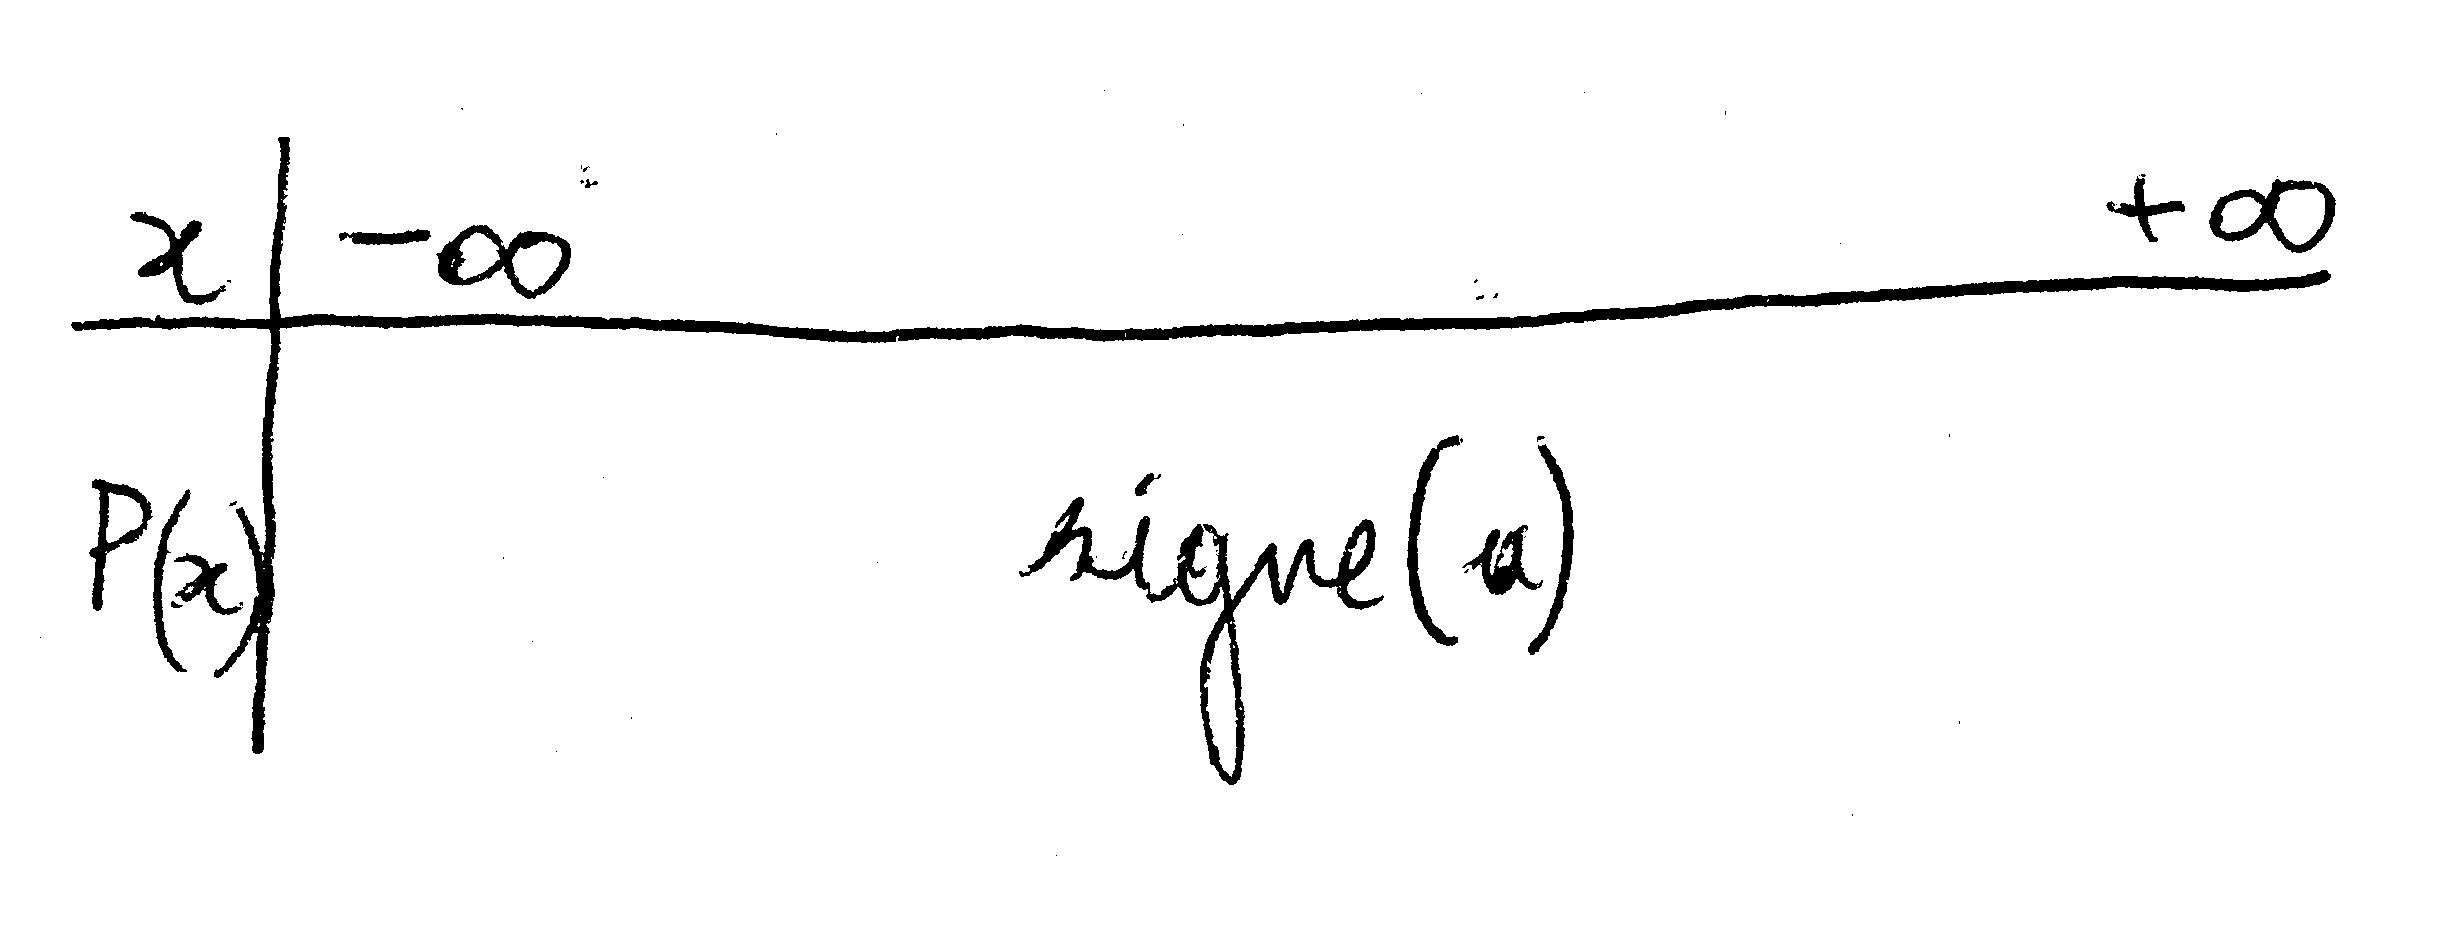
\includegraphics[width=0.4\textwidth]{pics/1.png}

\item si $\Delta = 0$, $P(x)$ est du signe de $a$ sur $\mathbb{R}$ et s'annule en $\frac{-b}{2a}$

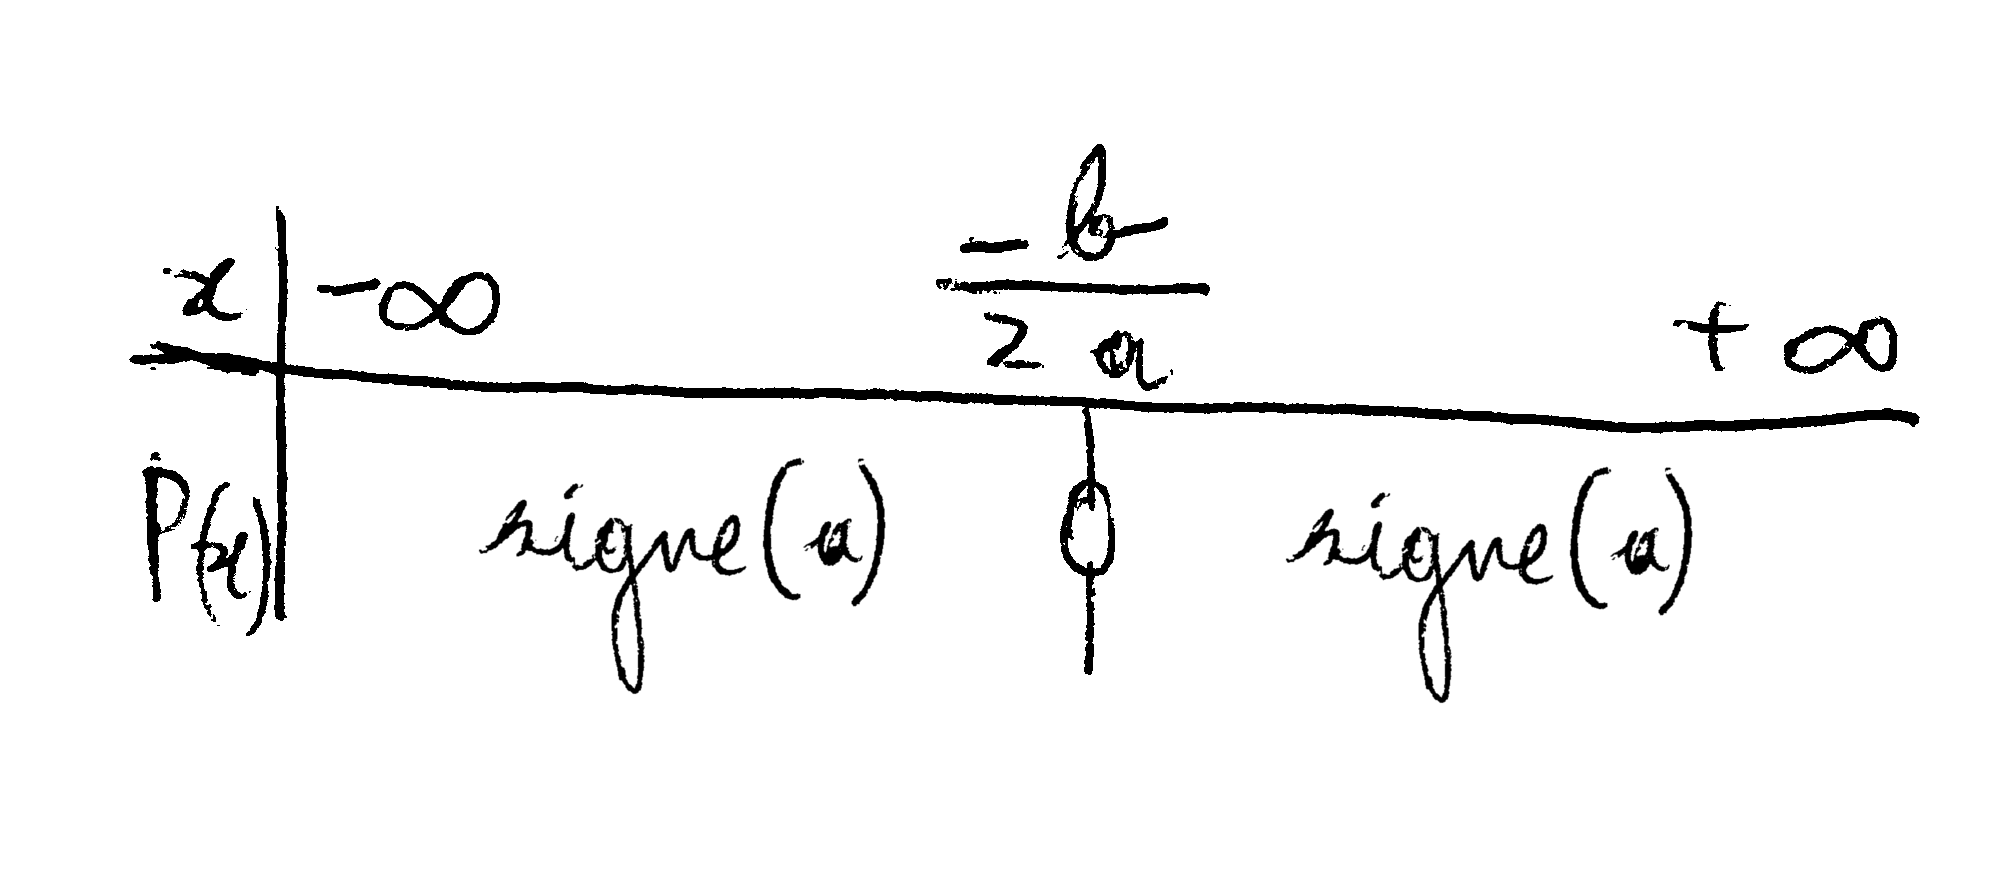
\includegraphics[width=0.4\textwidth]{pics/2.png}


\item si $\Delta > 0$ et que les racines sont $x_1$ et $x_2$, $P(x)$ est du signe de $-a$ sur $[x_1;x_2]$ \og entre les racines \fg{}  et du signe de $a$ sur $\mathbb{R} - ]x_1;x_2[ = ]-\infty ; x_1] \cup [x_2 ; +\infty[$ \og à l'extérieur des racines \fg{}.

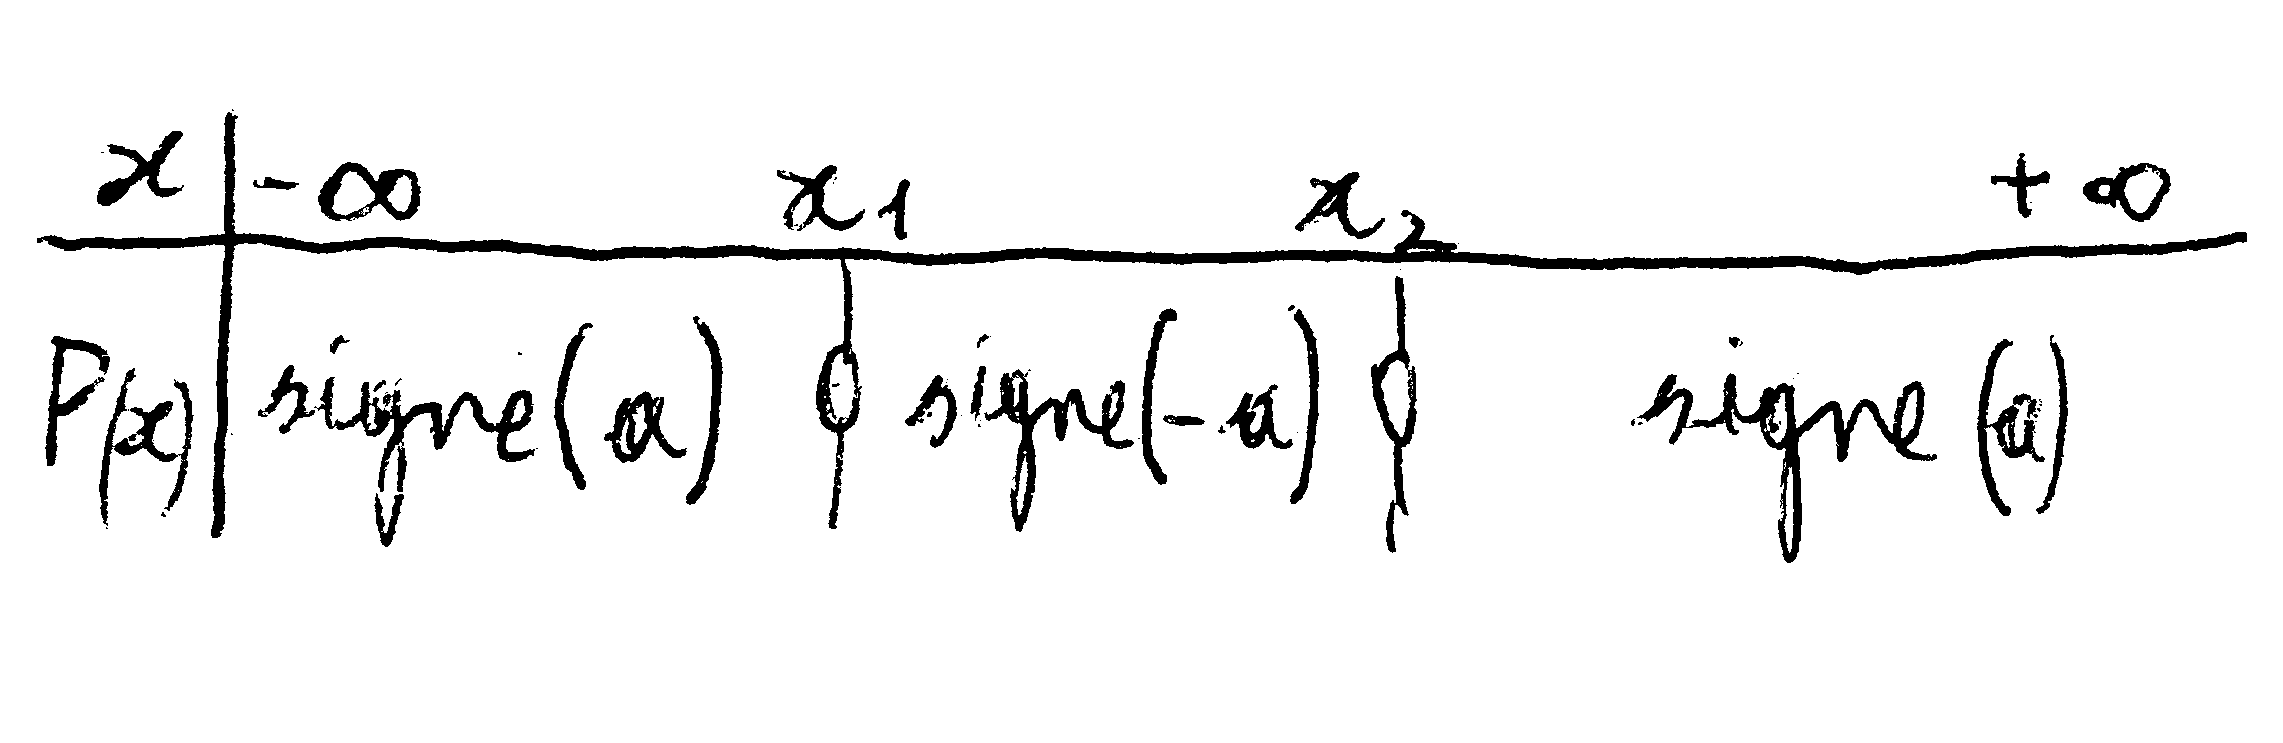
\includegraphics[width=0.4\textwidth]{pics/3.png}


\end{itemize}

\question{$x^2 + 5x + 1$}

$$\Delta = 5^2 - 4 \times 1 \times 1 = 21 > 0$$

Le polynôme a donc 2 racines.

$$\sqrt{\Delta} = \sqrt{21}$$

$$x_1 = \dfrac{-5 - \sqrt{21}}{2}$$

$$x_2 = \dfrac{-5 + \sqrt{21}}{2}$$

Le polynôme se factorise donc comme suit: $\left(x + \dfrac{5 + \sqrt{21}}{2}\right)\left(x + \dfrac{5 - \sqrt{21}}{2}\right)$

Tableau de signe:

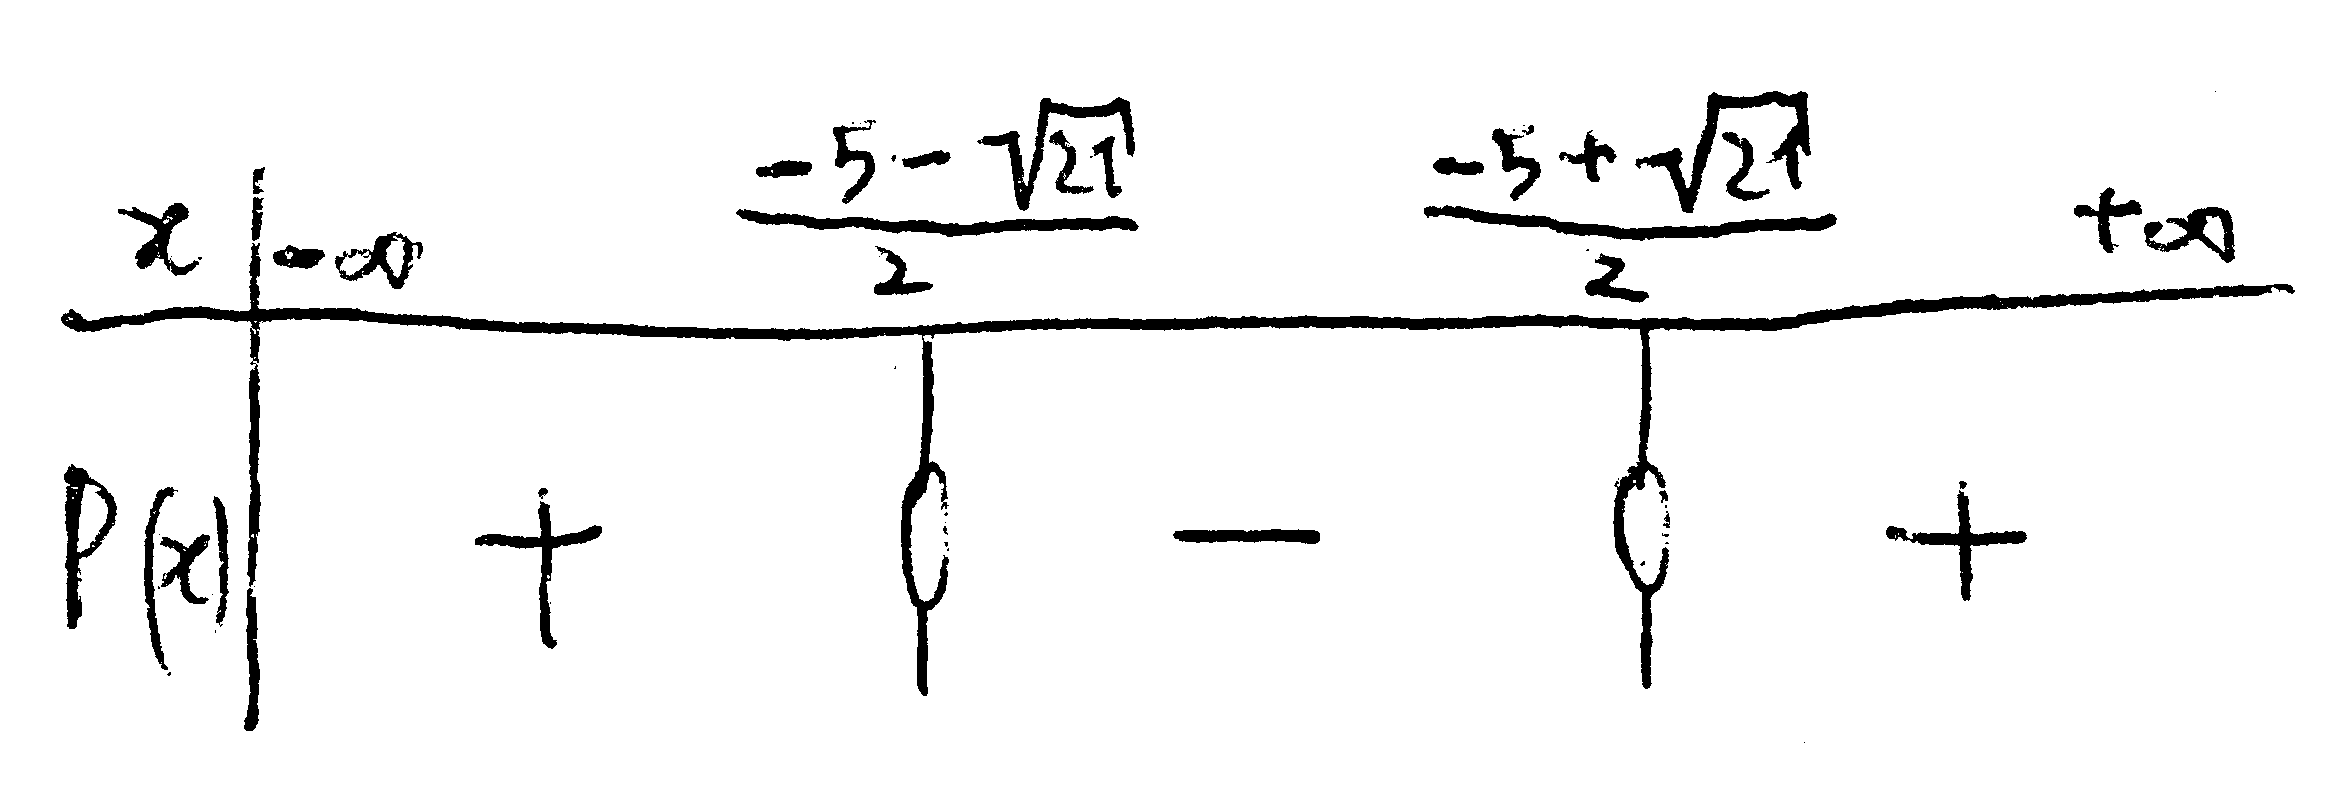
\includegraphics[width=0.4\textwidth]{pics/4.png}


\question{$x^2 + x + 5$}

$$\Delta = 1^2 - 4 \times 1 \times 5 = -19 < 0$$

Le polynôme n'a donc pas de racine réelle et ne peut donc pas se factoriser.

Tableau de signe:

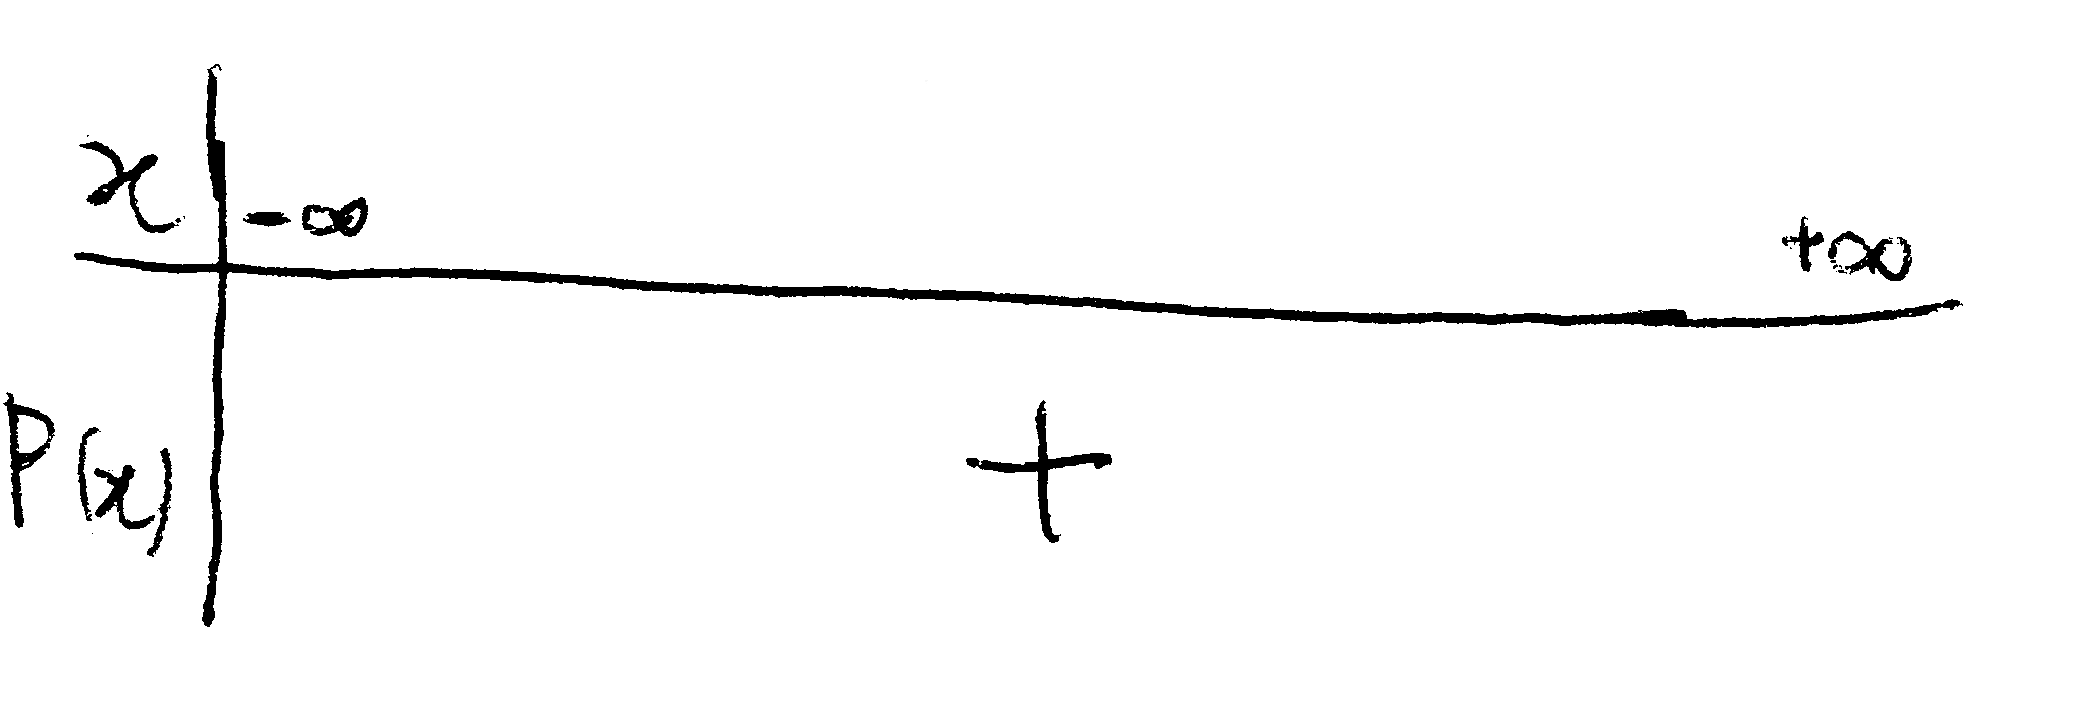
\includegraphics[width=0.4\textwidth]{pics/5.png}


\question{$7x^2 + 2x - 9$}

$$\Delta = 2^2 - 4 \times 7 \times (-9) = 256 > 0$$

Le polynôme a donc 2 racines.

$$\sqrt{\Delta} = 16$$

$$x_1 = \dfrac{-2 - 16}{14} = -\dfrac{9}{7}$$

$$x_2 = \dfrac{-2 + 16}{14} = 1$$

Le polynôme se factorise donc comme suit: $7\left(x + \dfrac{9}{7}\right)\left(x -1\right)$

Tableau de signe:

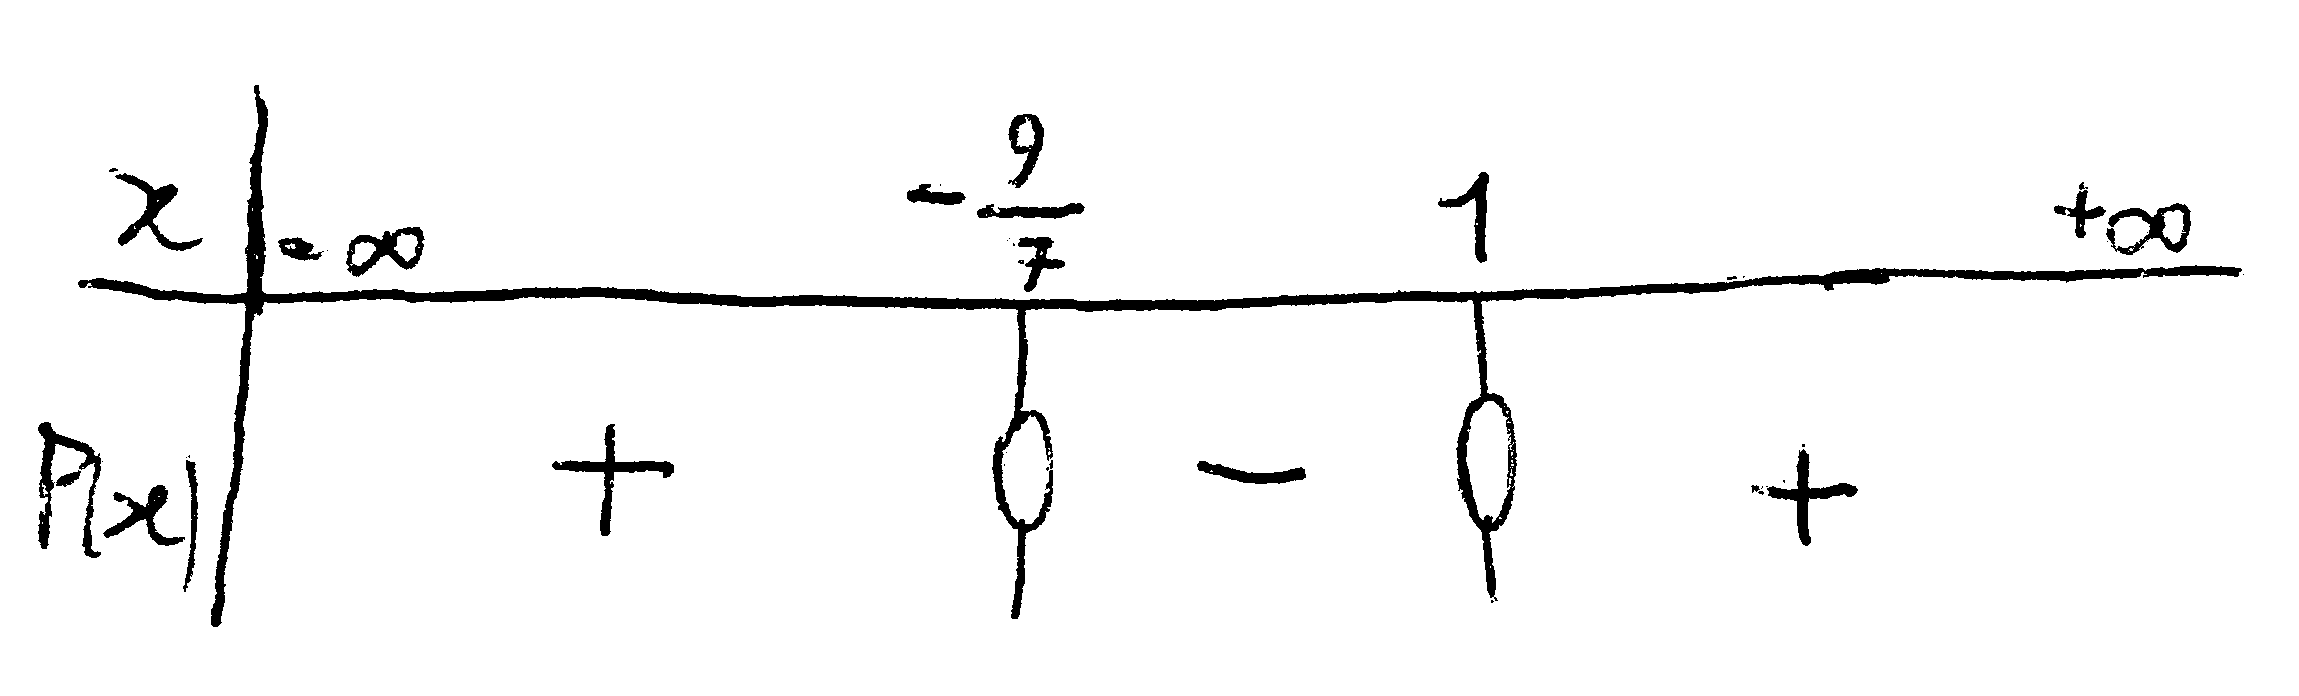
\includegraphics[width=0.4\textwidth]{pics/6.png}


\question{$2x^2 - 9x + 4$}

$$\Delta = (-9)^2 - 4 \times 2 \times 4 = 65 > 0$$

Le polynôme a donc 2 racines.

$$\sqrt{\Delta} = \sqrt{65}$$

$$x_1 = \dfrac{9 - \sqrt{65}}{4}$$

$$x_2 = \dfrac{9 + \sqrt{65}}{4}$$

Le polynôme se factorise donc comme suit: $2\left(x - \dfrac{9 + \sqrt{65}}{4}\right)\left(x - \dfrac{9 - \sqrt{65}}{4}\right)$

Tableau de signe:

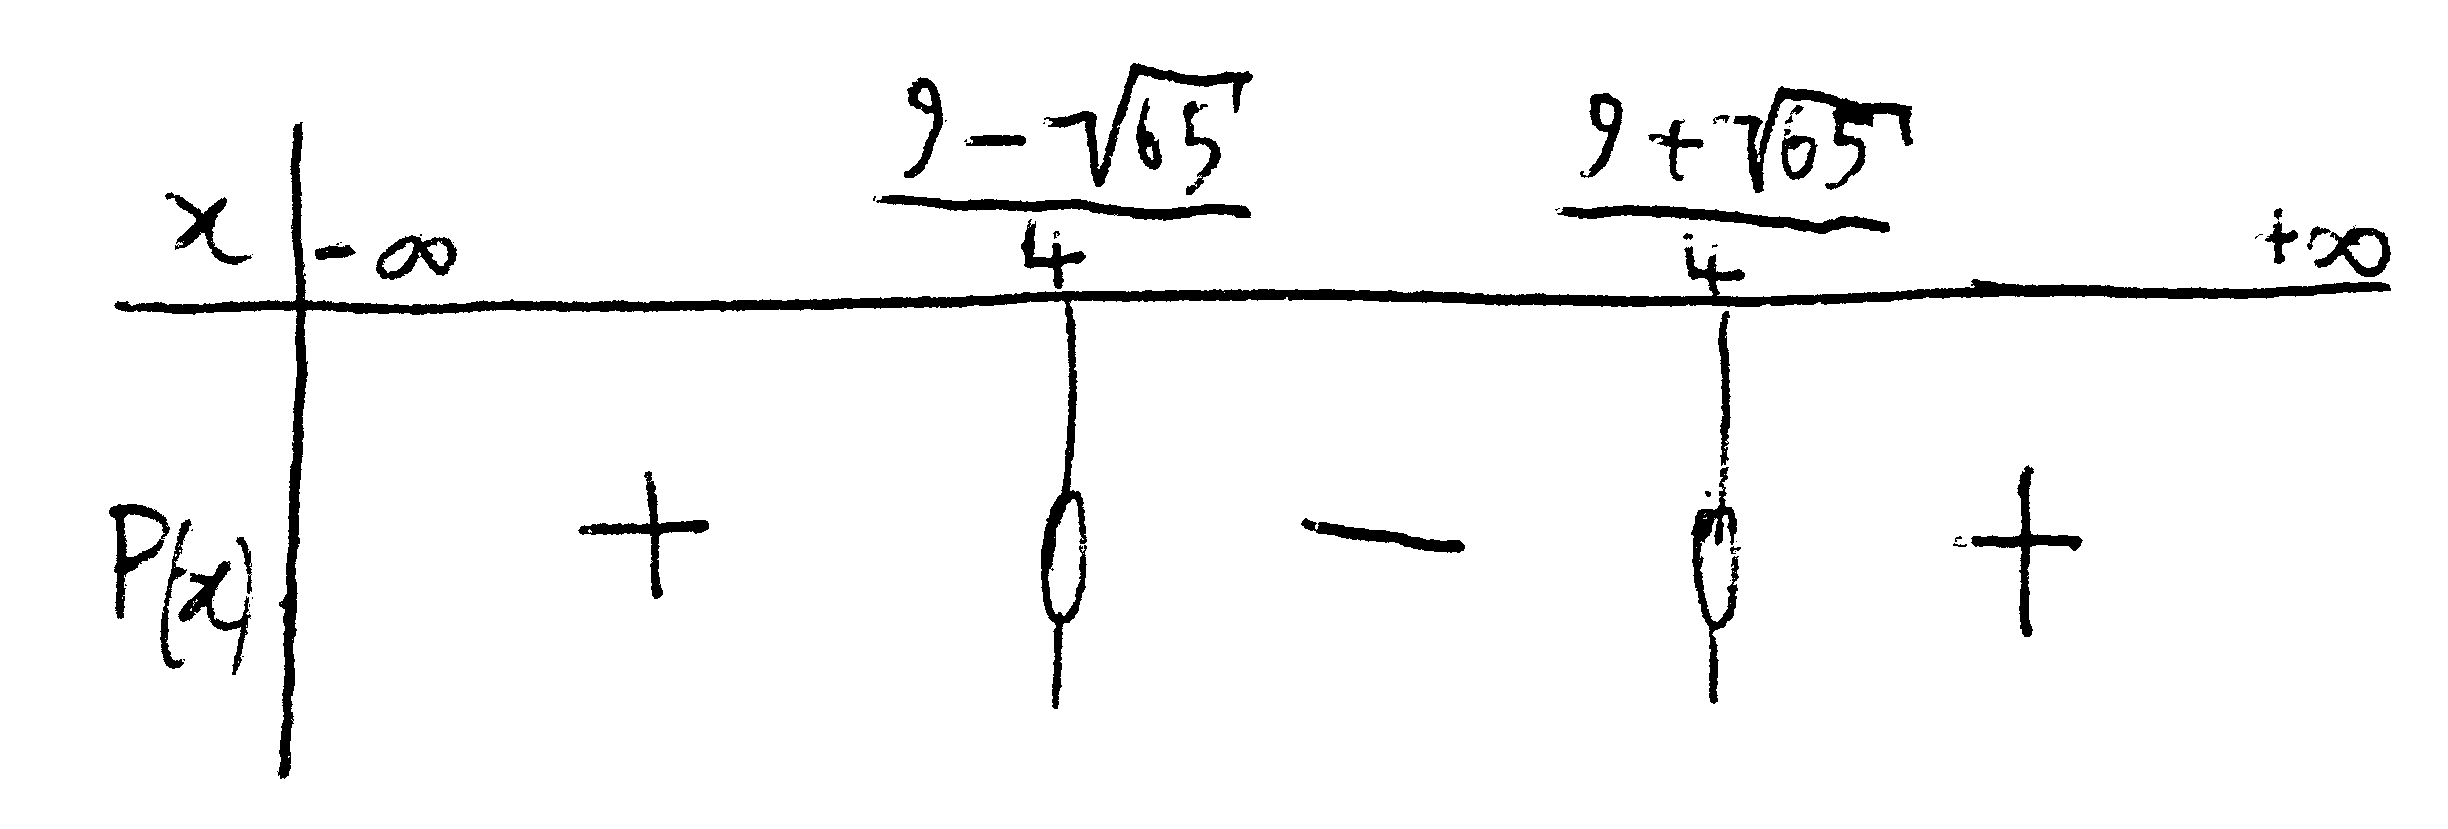
\includegraphics[width=0.4\textwidth]{pics/7.png}


\question{$2x^2 + 8x + 9$}

$$\Delta = 8^2 - 4 \times 2 \times 9 = -8 < 0$$

Le polynôme n'a donc pas de racine. Il ne se factorise pas.

Tableau de signe:

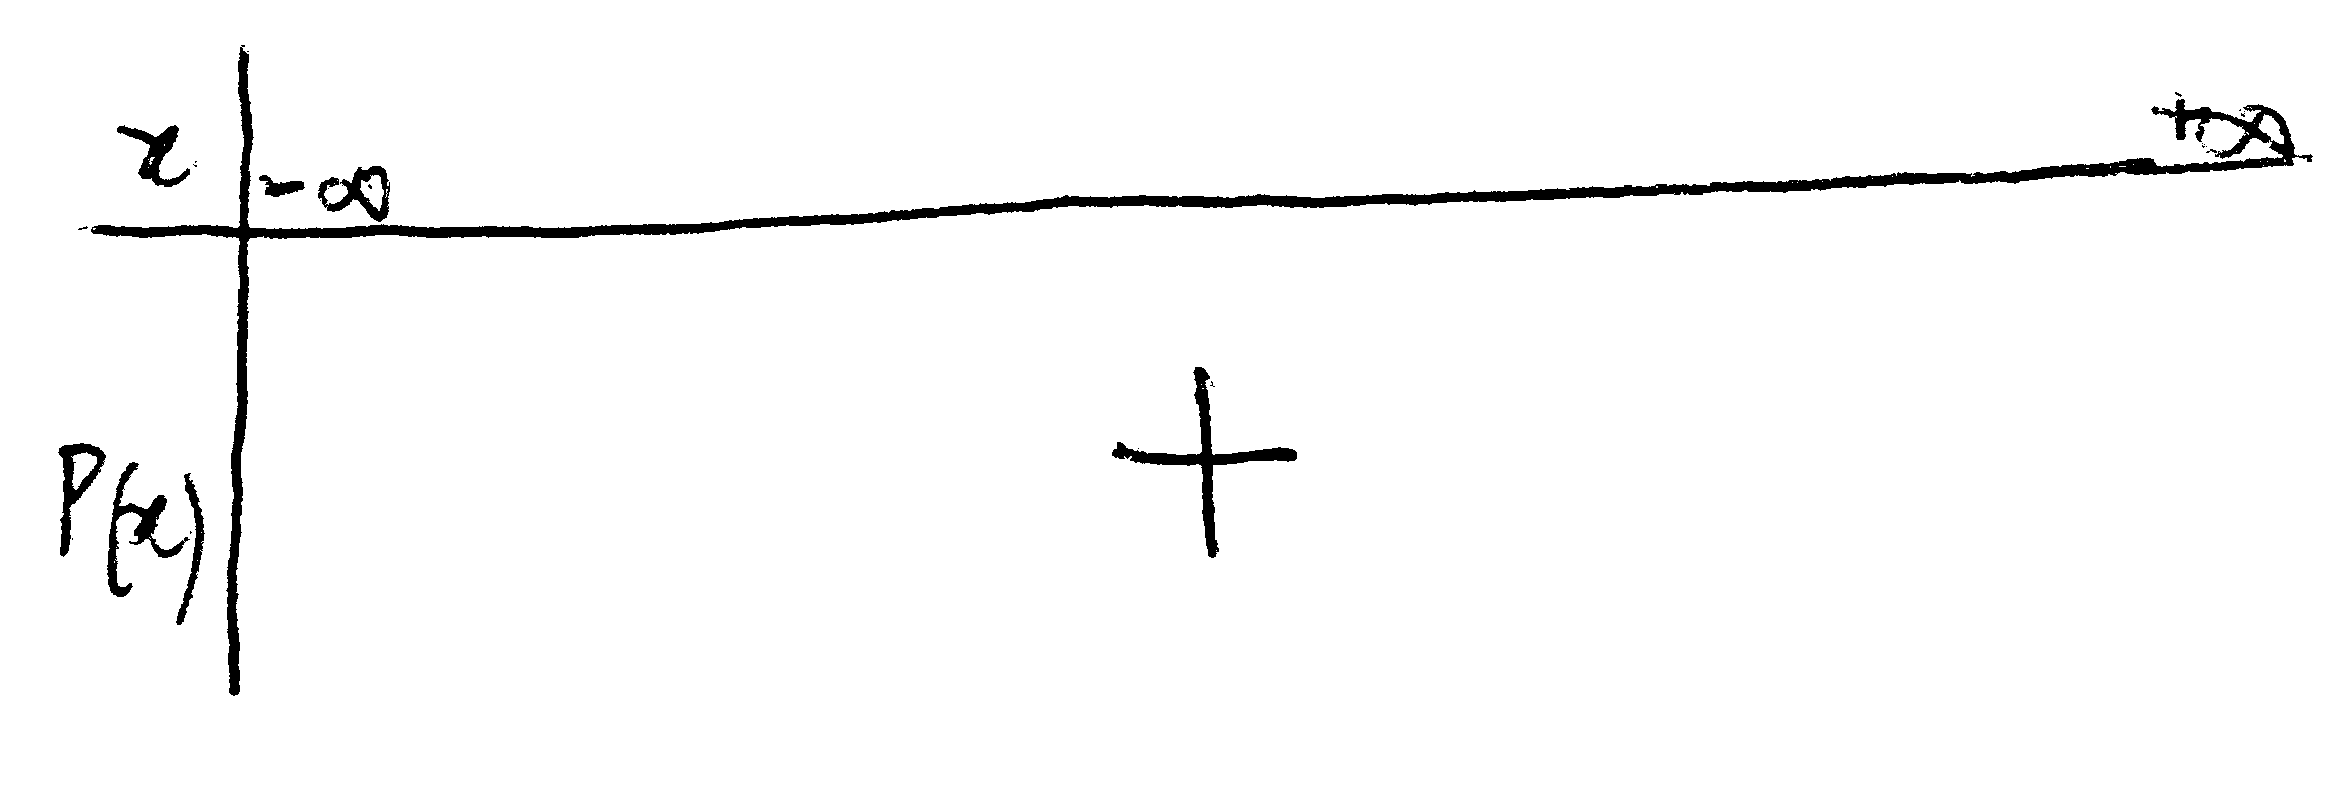
\includegraphics[width=0.4\textwidth]{pics/8.png}


\question{$2x^2 + 3x + 2$}

$$\Delta = 3^2 - 4 \times 2 \times 2 = -7 < 0$$

Le polynôme n'a donc pas de racine. Il ne se factorise pas.

Tableau de signe:

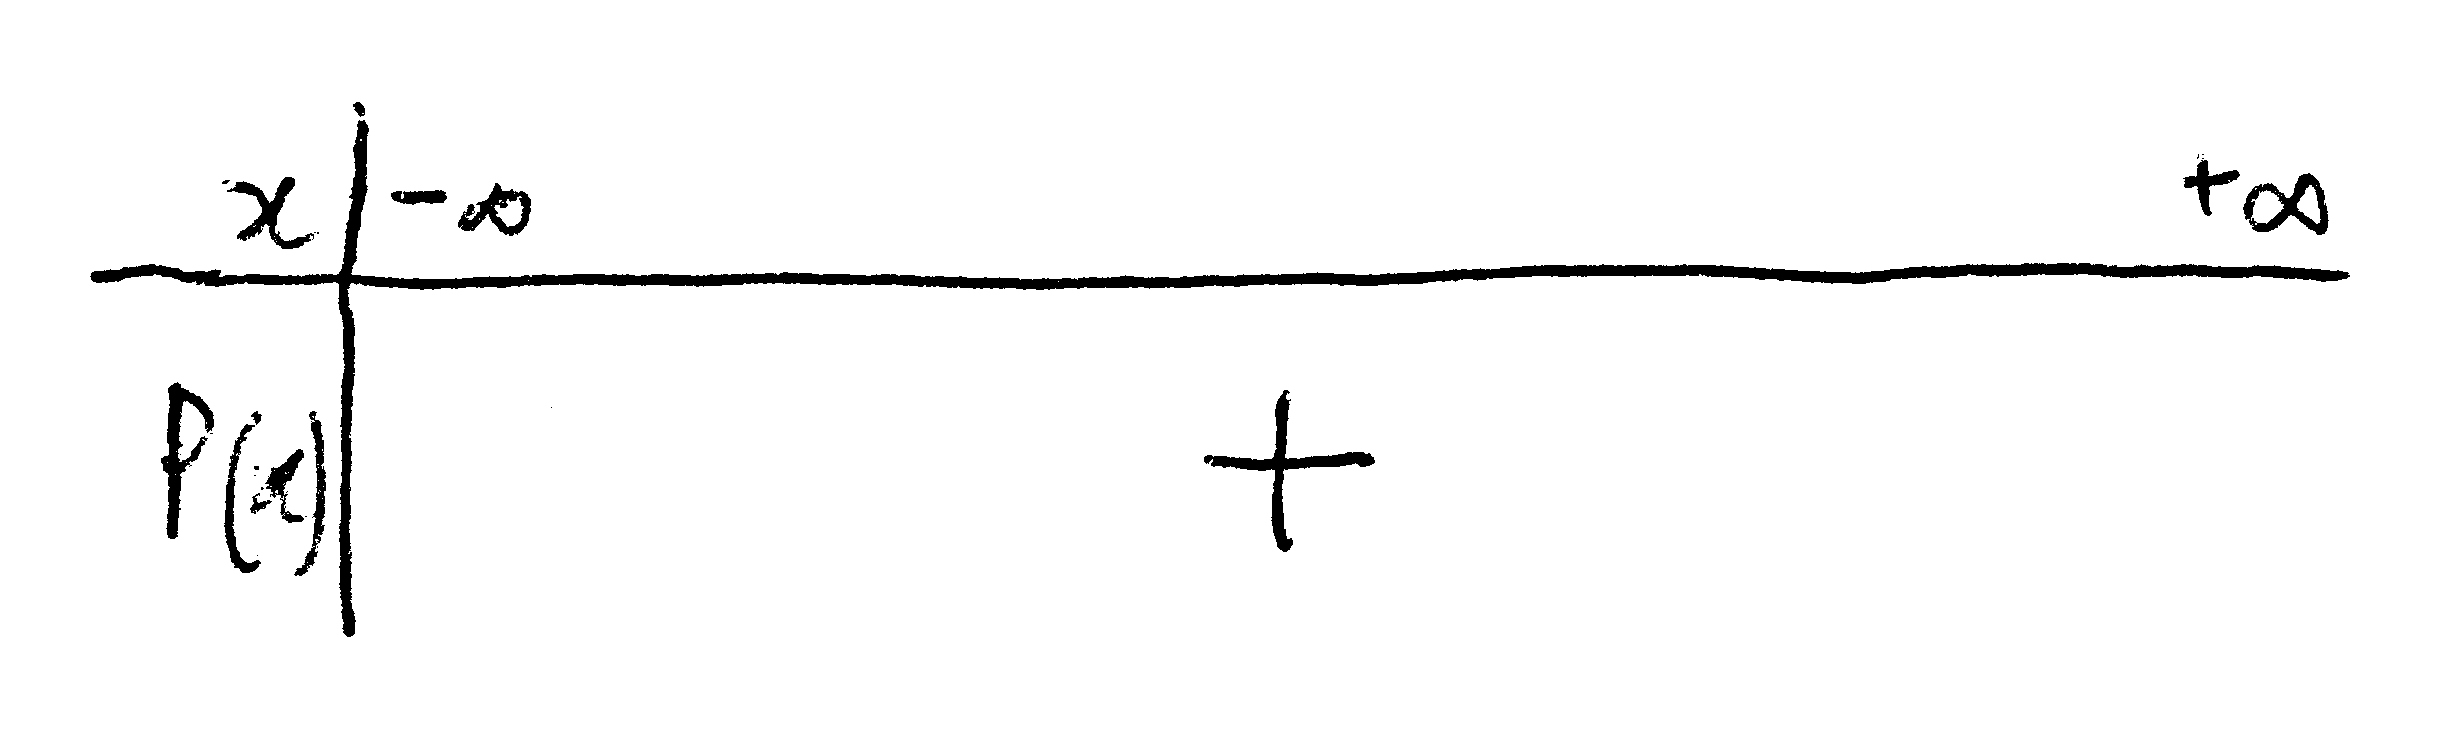
\includegraphics[width=0.4\textwidth]{pics/9.png}


\question{$x^2 + 12x + 11$}

$$\Delta = 12^2 - 4 \times 2 \times 11 = 100 > 0$$

Le polynôme a donc 2 racines.

$$\sqrt{\Delta} = 10$$

$$x_1 = \dfrac{-12 - 10}{2} = -11$$

$$x_2 = \dfrac{-12 + 10}{2} = -1$$

Le polynôme se factorise donc comme suit: $\left(x + 11\right)\left(x + 1\right)$

Tableau de signe:

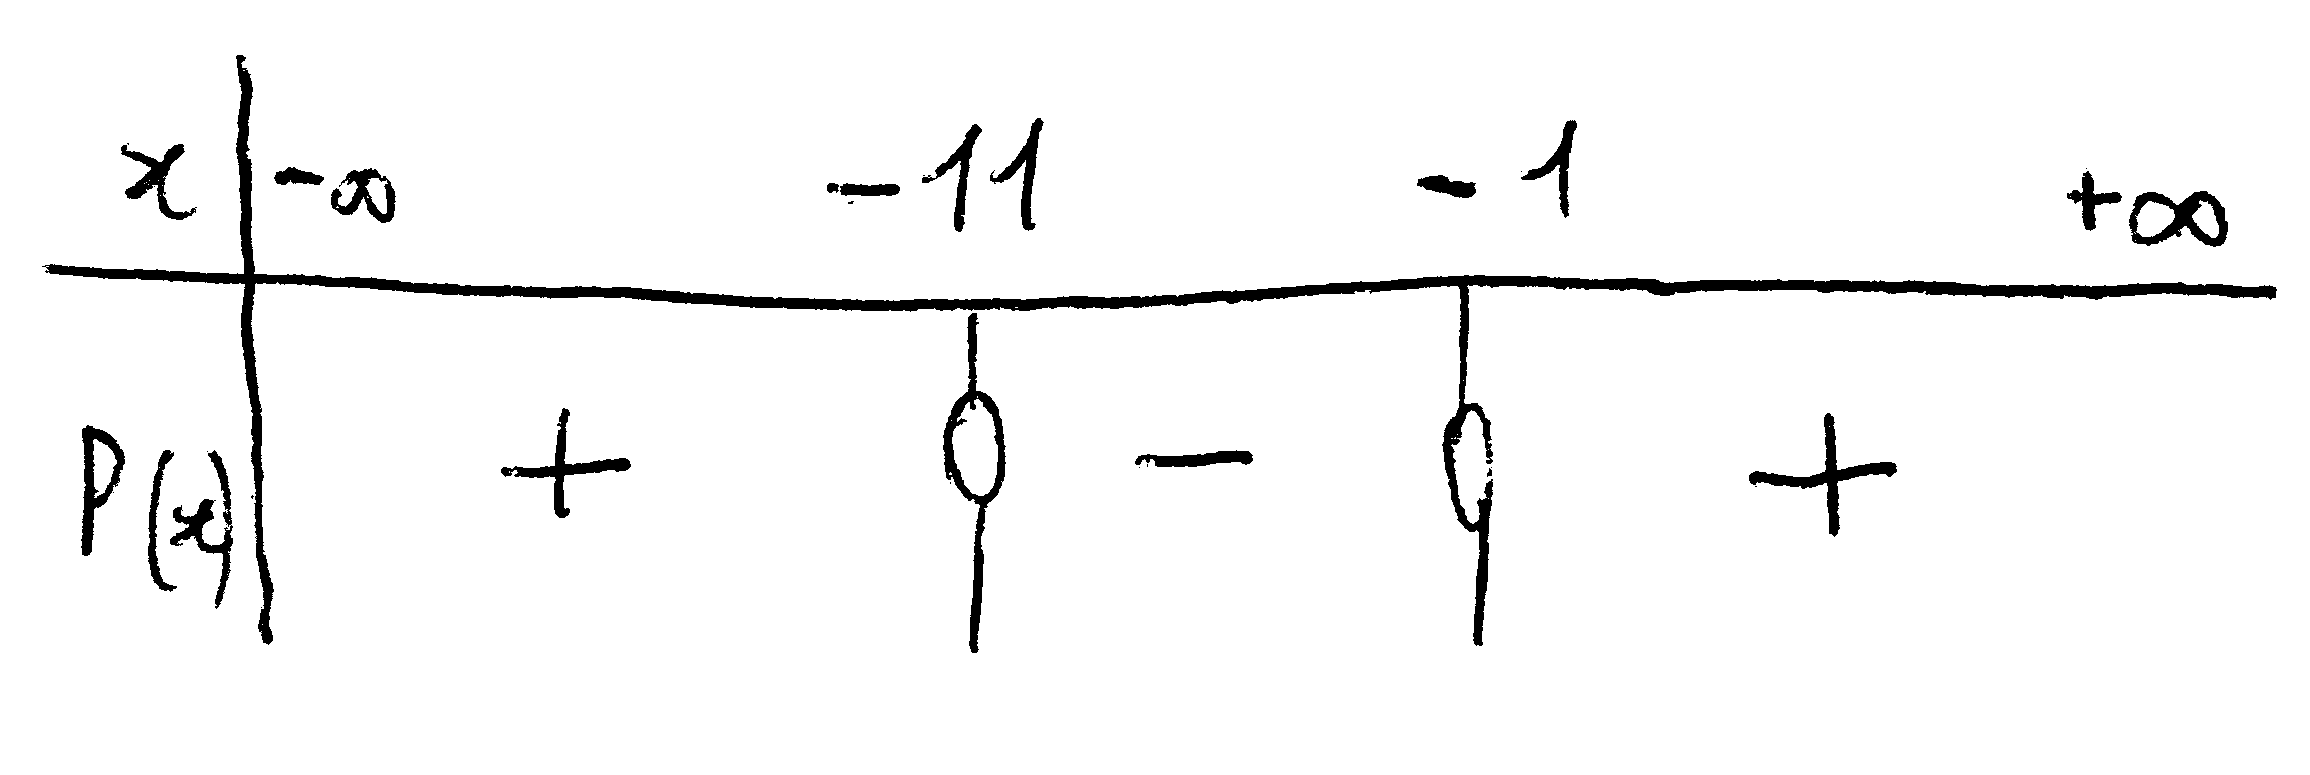
\includegraphics[width=0.4\textwidth]{pics/10.png}


\question{$8x^2 - 10x + 3$}

$$\Delta = (-10)^2 - 4 \times 8 \times 3 = 4 > 0$$

Le polynôme a donc 2 racines.

$$\sqrt{\Delta} = 2$$

$$x_1 = \dfrac{10 - 2}{16} = \dfrac{1}{2}$$

$$x_2 = \dfrac{10 + 2}{16} = \dfrac{3}{4}$$

Le polynôme se factorise donc ainsi: $8\left(x - \dfrac{1}{2}\right)\left(x - \dfrac{3}{4}\right)$

Tableau de signe:

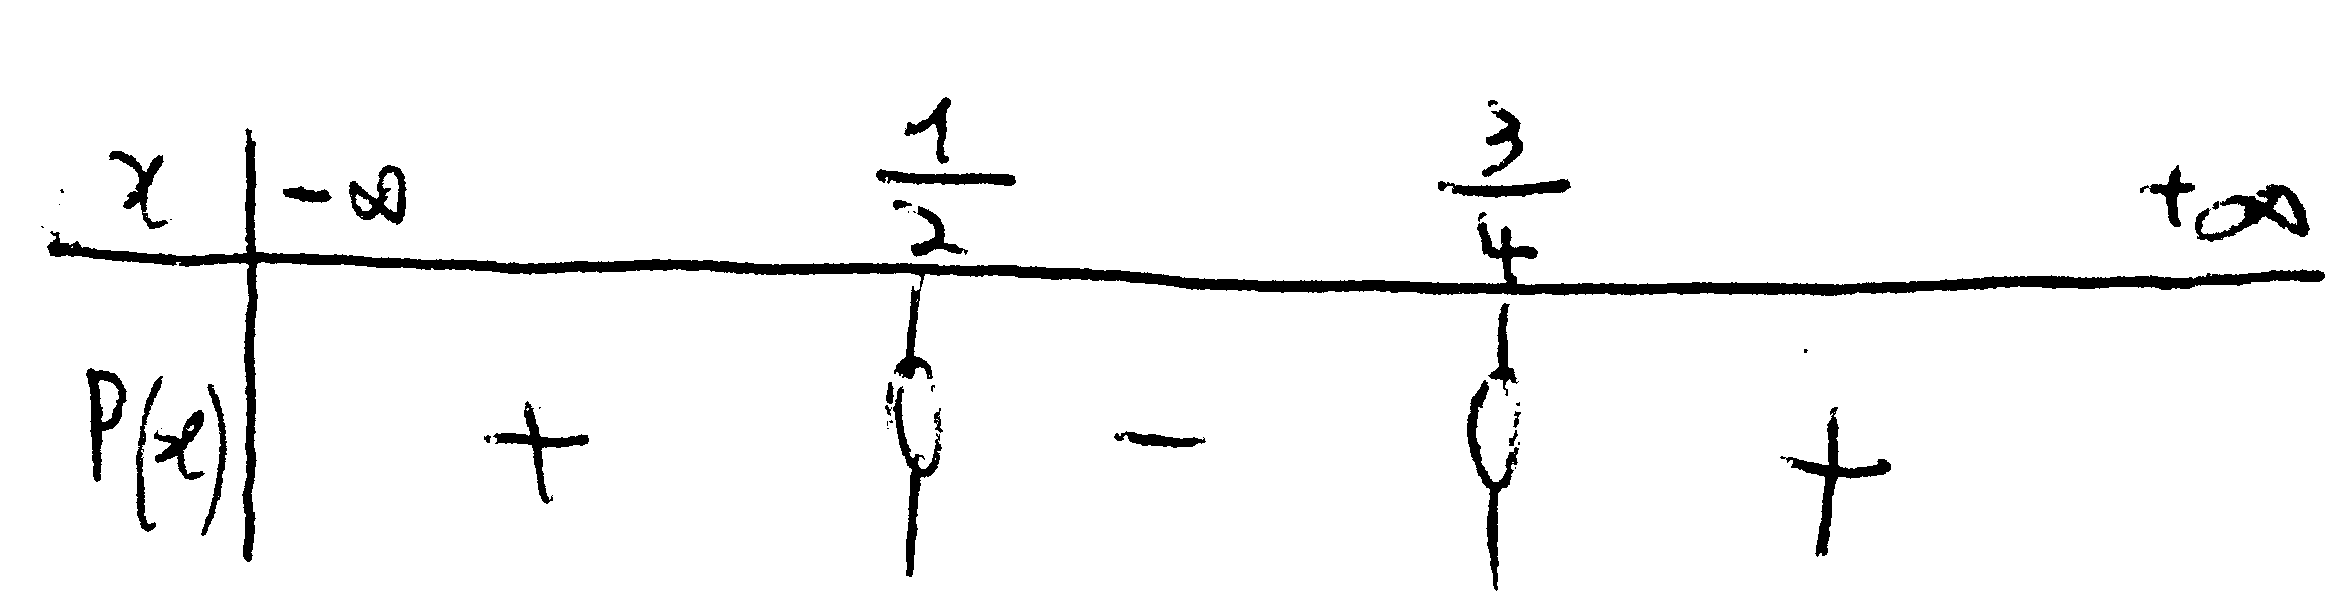
\includegraphics[width=0.4\textwidth]{pics/11.png}


\question{$2x^2 + 7x + 6$}

$$\Delta = 7^2 - 4 \times 2 \times 6 = 1 > 0$$

Le polynôme a donc 2 racines.

$$\sqrt{\Delta} = 1$$

$$x_1 = \dfrac{-7 - 1}{4} = -2$$

$$x_2 = \dfrac{-7 + 1}{4} = -\dfrac{3}{2}$$

Le polynôme se factorise donc de la façon suivante: $2\left(x + 2\right)\left(x + \dfrac{3}{2}\right)$

Tableau de signe:

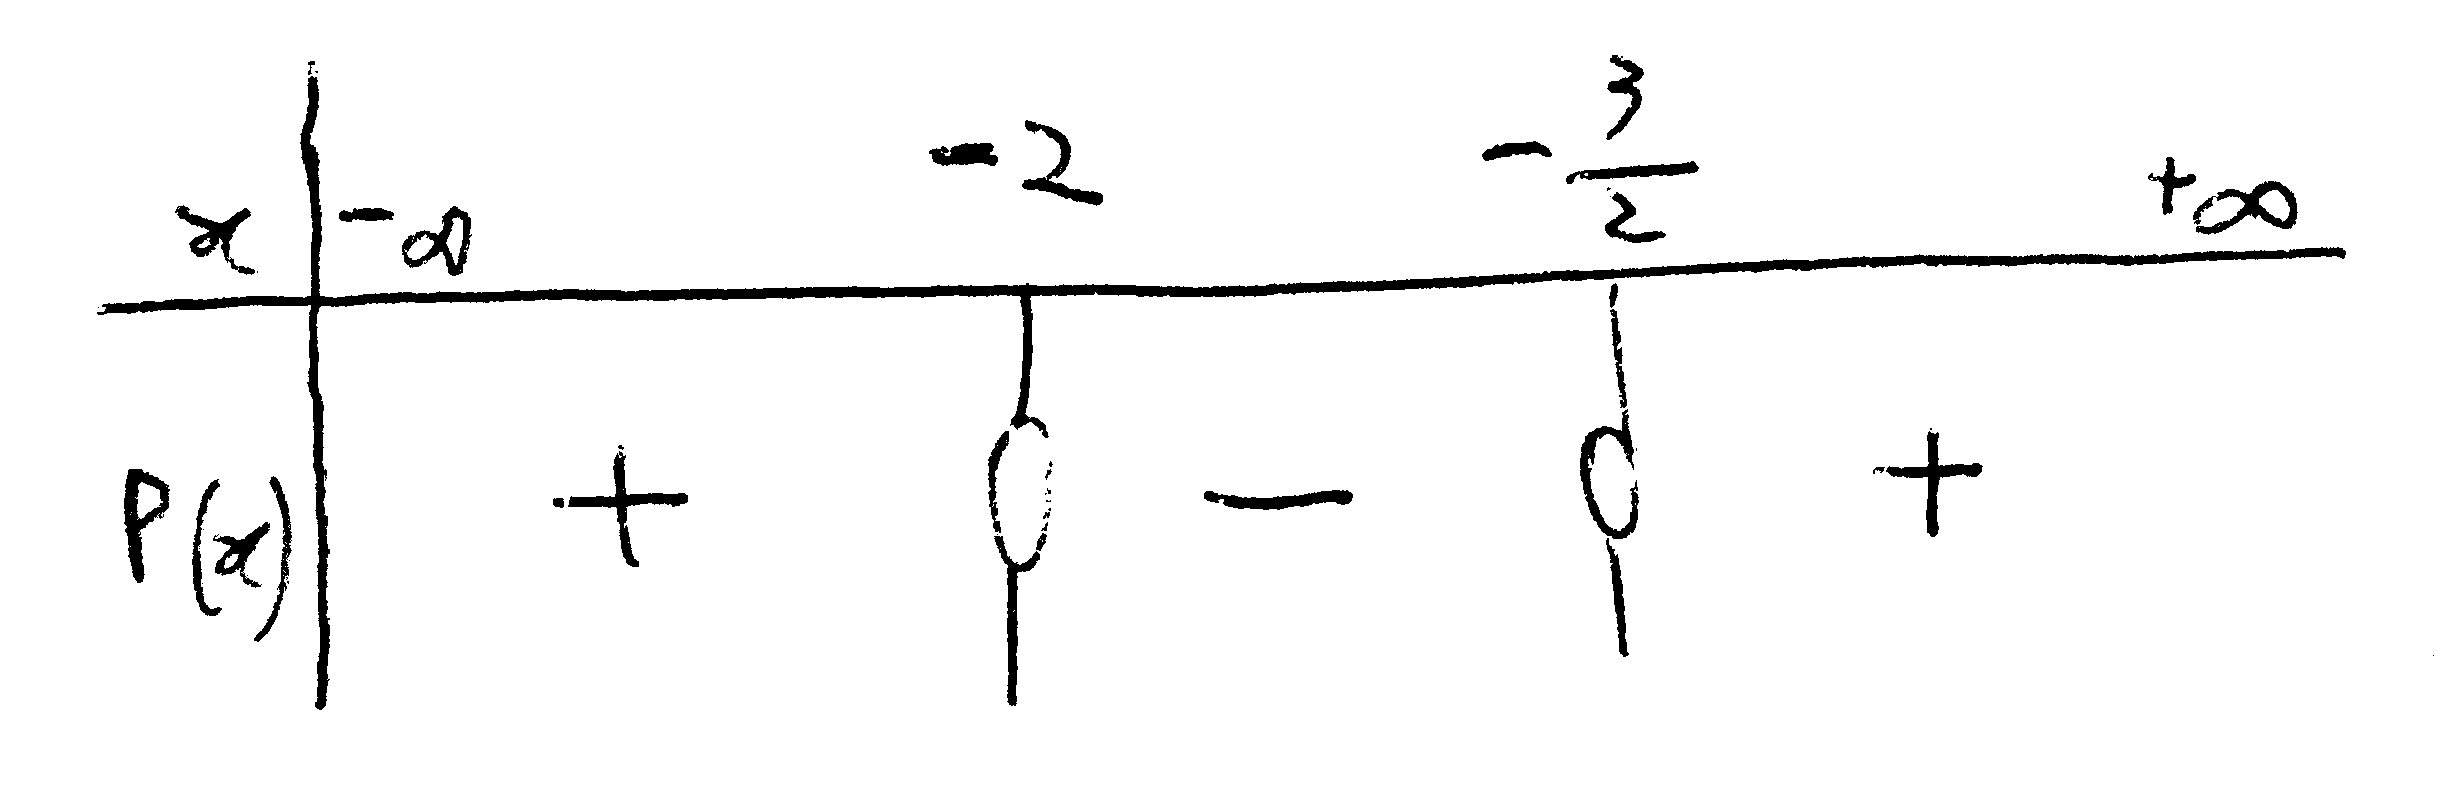
\includegraphics[width=0.4\textwidth]{pics/12.png}


\question{$-x^2 + 4x - 4$}

$$\Delta = 4^2 - 4 \times (-1) \times (-4) = 0$$

L'équation $-x^2 + 4x - 4 = 0$ a donc une seule solution.

$$x_1 = \dfrac{-4}{-2} = 2$$

Le polynôme se factorise donc ainsi: $-\left(x - 2\right)^2$

Tableau de signe:

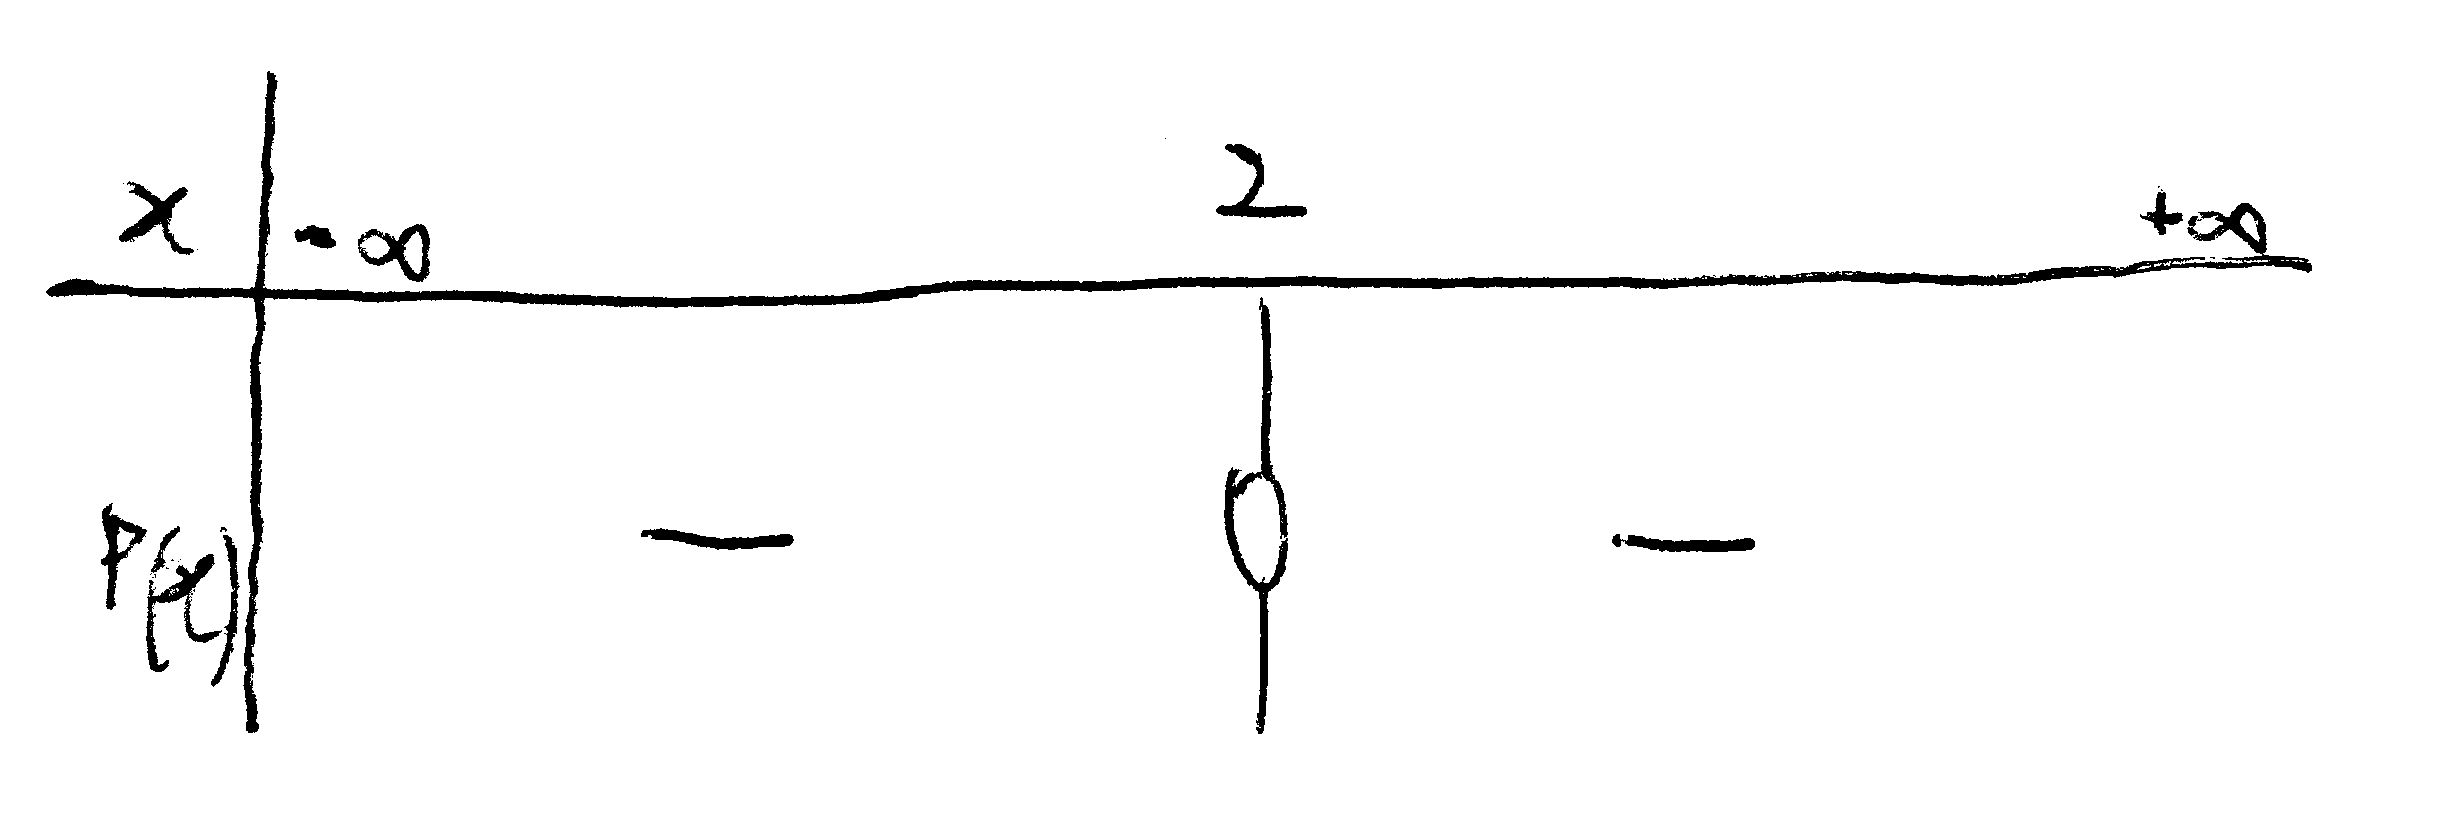
\includegraphics[width=0.4\textwidth]{pics/13.png}


\section*{Équations, inéquations}

\exo{Résoudre ces équations:}

\question{$2x + 4 = -x + 2$}

$$\Leftrightarrow 3x = -2 \Leftrightarrow x = -\dfrac{2}{3}$$

$$S = \left\{ -\dfrac{2}{3} \right\}$$

\question{$8x^2 + 9x + 12 = -9x^2 - 5x + 16$}

On remarque qu'on a de part et d'autre du signe $=$ deux polynômes du second degré. Pensez que dans ce cas, en faisant passer l'un des 2 de l'autre côté, on a toujours un polynôme du second degré, dont on pourra calculer les racines:

$$8x^2 + 9x + 12 = -9x^2 - 5x + 16$$

$$\Leftrightarrow 17x^2 + 14x - 4 = 0$$

$$\Delta = 14^2 - 4 \times 17 \times (-4) = 468 > 0$$

Le polynôme a donc 2 racines.

$$\sqrt{\Delta} = \sqrt{468} = \sqrt{4 \times 9 \times 13} = 6\sqrt{13}$$

$$x_1 = \dfrac{-14 - 6\sqrt{13}}{34} = \dfrac{-7 - 3\sqrt{13}}{17}$$

$$x_2 = \dfrac{-14 + 6\sqrt{13}}{34} = \dfrac{-7 + 3\sqrt{13}}{17}$$

$$S = \left\{ \dfrac{-7 - 3\sqrt{13}}{17} ; \dfrac{-7 + 3\sqrt{13}}{17} \right\}$$

\question{$\dfrac{x}{4} + 2 = x + 4$}

$$\Leftrightarrow \dfrac{x}{4} - x = 2$$

$$\Leftrightarrow -\dfrac{3}{4}x = 2$$

$$\Leftrightarrow x = -2 \times \dfrac{4}{3} = -\dfrac{8}{3}$$

$$S = \left\{ -\dfrac{8}{3}\right\}$$


\question{$\dfrac{2x + 4}{6}  = \dfrac{7x + 1}{12}$}

On met au même dénominateur:

$$\Leftrightarrow \dfrac{4x + 8}{12}  = \dfrac{7x + 1}{12}$$

$$\Leftrightarrow 4x + 8 = 7x + 1$$

$$\Leftrightarrow 7 = 3x$$

$$\Leftrightarrow x = \dfrac{7}{3}$$

$$S = \left\{ \dfrac{7}{3}\right\}$$

\question{$x^2 + 8x = -12$}

$$\Leftrightarrow x^2 + 8x + 12 = 0$$

On reconnaît ici un polynôme du 2\textsuperscript{nd} degré.

$$\Delta = 8^2 - 4 \times 12 = 16 > 0$$

L'équation a donc 2 solutions.

$$\sqrt{\Delta} = 4$$

$$x_1 = \dfrac{-8 - 4}{2} = -6$$

$$x_2 = \dfrac{-8 + 4}{2} = -2$$

On obtient donc $S = \left\{ -6;-2\right\}$

\question{$2x^2 = -1$}

On sait que pour tout réel $x$, $x^2 \geqslant 0$, donc $2x^2 \geqslant 0$

L'équation $2x^2 = -1$ n'a donc pas de solution.

$$S = \emptyset$$

\question{$\dfrac{1-x}{x-1} = 3$}

On remarque que la fraction peut avoir des valeurs interdites. Vérifions en résolvant l'équation \og{}$\mbox{dénominateur} = 0$ \fg{}   soit $x-1 = 0$:

$x-1 = 0 \Leftrightarrow x = 1$. 

1 est valeur interdite, on résout donc sur $\mathbb{R} - \{1\}$ ($\mathbb{R}$ privé de 1). On obtient donc:

$\dfrac{1-x}{x-1} = 3 \Leftrightarrow 3(x-1) = 1-x$ pour $x \neq 1$

$\Leftrightarrow 4x = 4 \Leftrightarrow x=1$ pour $x \neq 1$.

L'unique solution que l'on trouve est 1, mais elle ne fait pas partie de l'ensemble de définition de $\dfrac{1-x}{x-1}$.

$$S = \emptyset$$


\question{$(x-2)(x^2 + 4x + 3) = 0$}

On remarque ici qu'on a un produit. L'équation est donc équivalente à :

$$
\begin{cases} 
x-2 &= 0 \\
\mbox{ou} & \\
x^2 + 4x + 3 &= 0
\end{cases}
$$

On résout la première équation: $x - 2 = 0 \Leftrightarrow x = 2$

puis la seconde:

$$x^2 + 4x + 3 = 0$$

On reconnaît un polynôme du second degré.

$$\Delta = 4^2 - 4 \times 1 \times 3 = 4 > 0$$

L'équation a donc 2 solutions.

$$\sqrt{\Delta} = 2$$

$$x_1 = \dfrac{-4 - 2}{2} = -3$$

$$x_2 = \dfrac{-4 + 2}{2} = -1$$

On réunit les solutions obtenues pour les deux équations et obtient: 

$$S = \left\{ 2 \right\} \cup \left\{ -2 ; -1 \right\} = \left\{ -2 ; -1 ; 2 \right\}$$

\exo{Et maintenant, ces inéquations:}

\question{$x + 2 \geqslant -x-1$}

$$\Leftrightarrow 2x \geqslant -3$$

$$\Leftrightarrow x \geqslant -\dfrac{3}{2}$$

$$S = \left[ -\dfrac{3}{2} ; +\infty \right]$$

\question{$4x + 1 \geqslant 2x - 3$}

$$\Leftrightarrow 2x \geqslant -4$$

$$\Leftrightarrow x \geqslant -2$$

$$S = \left[ -2 ; +\infty \right]$$

\question{$x^2 \leqslant 1$}

$$\Leftrightarrow x^2 - 1 \leqslant 0$$

$$\Leftrightarrow (x + 1)(x - 1) \leqslant 0$$

On peut donc dresser le tableau de signe suivant:

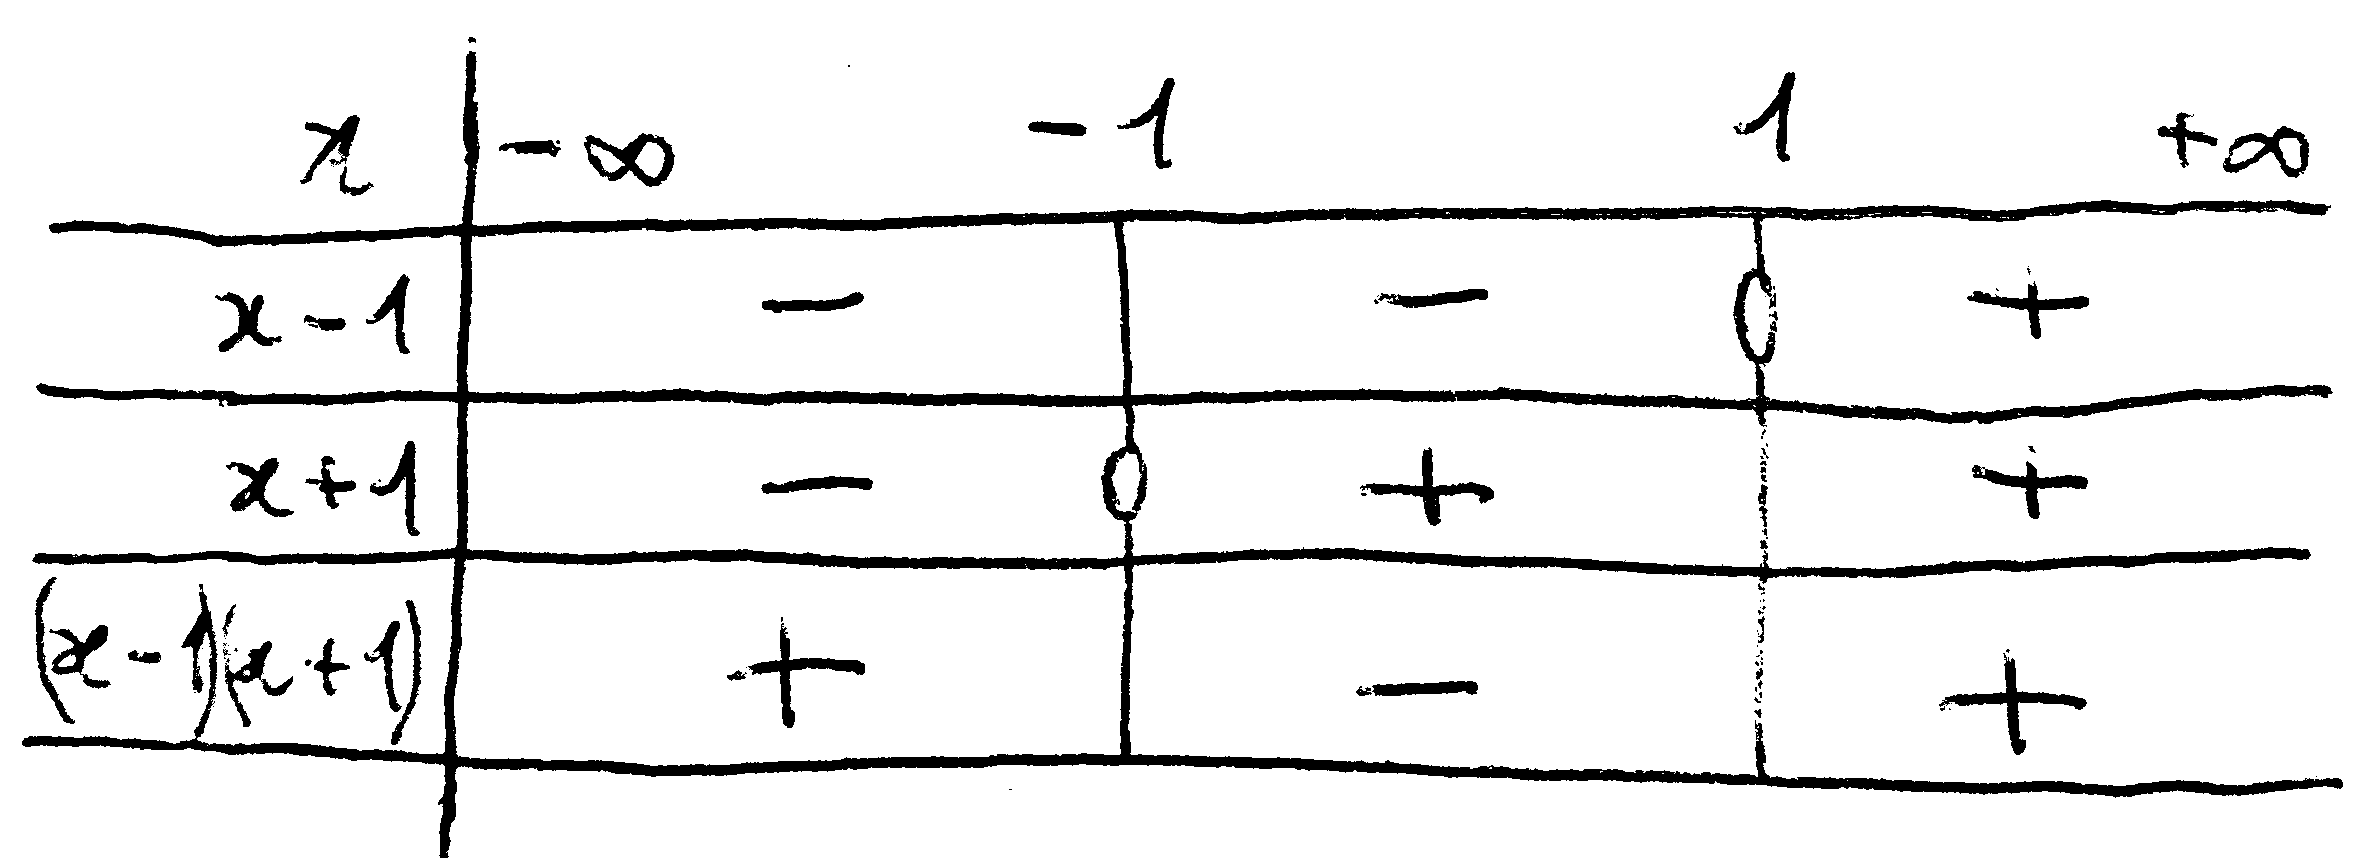
\includegraphics[width=0.4\textwidth]{pics/14.png}

D'où: $S = \left[ -1 ; 1 \right]$

\question{$2x \geqslant 12 + x$}

$$\Leftrightarrow x  \geqslant 12$$

$$S = \left[ 12 ; +\infty \right]$$

\question{$x+1 \leqslant x$}

$$\Leftrightarrow x-x+1 \leqslant 0 \Leftrightarrow 1 \leqslant 0$$

On remarque que ceci est impossible, quel que soit $x$. L'inéquation n'a donc pas de solution.

$$S = \emptyset$$

\question{$4(x+1)(x-2) \leqslant 0$}

Il s'agit d'un produit dont on veut connaître le signe. Nous allons donc étudier le signe de chacun des facteurs:

$$x+1 \geqslant 0 \Leftrightarrow x \geqslant -1$$

$$x-2 \geqslant 0 \Leftrightarrow x \geqslant 2$$

et $4 > 0$.

On peut donc en déduire le tableau de signe suivant: 

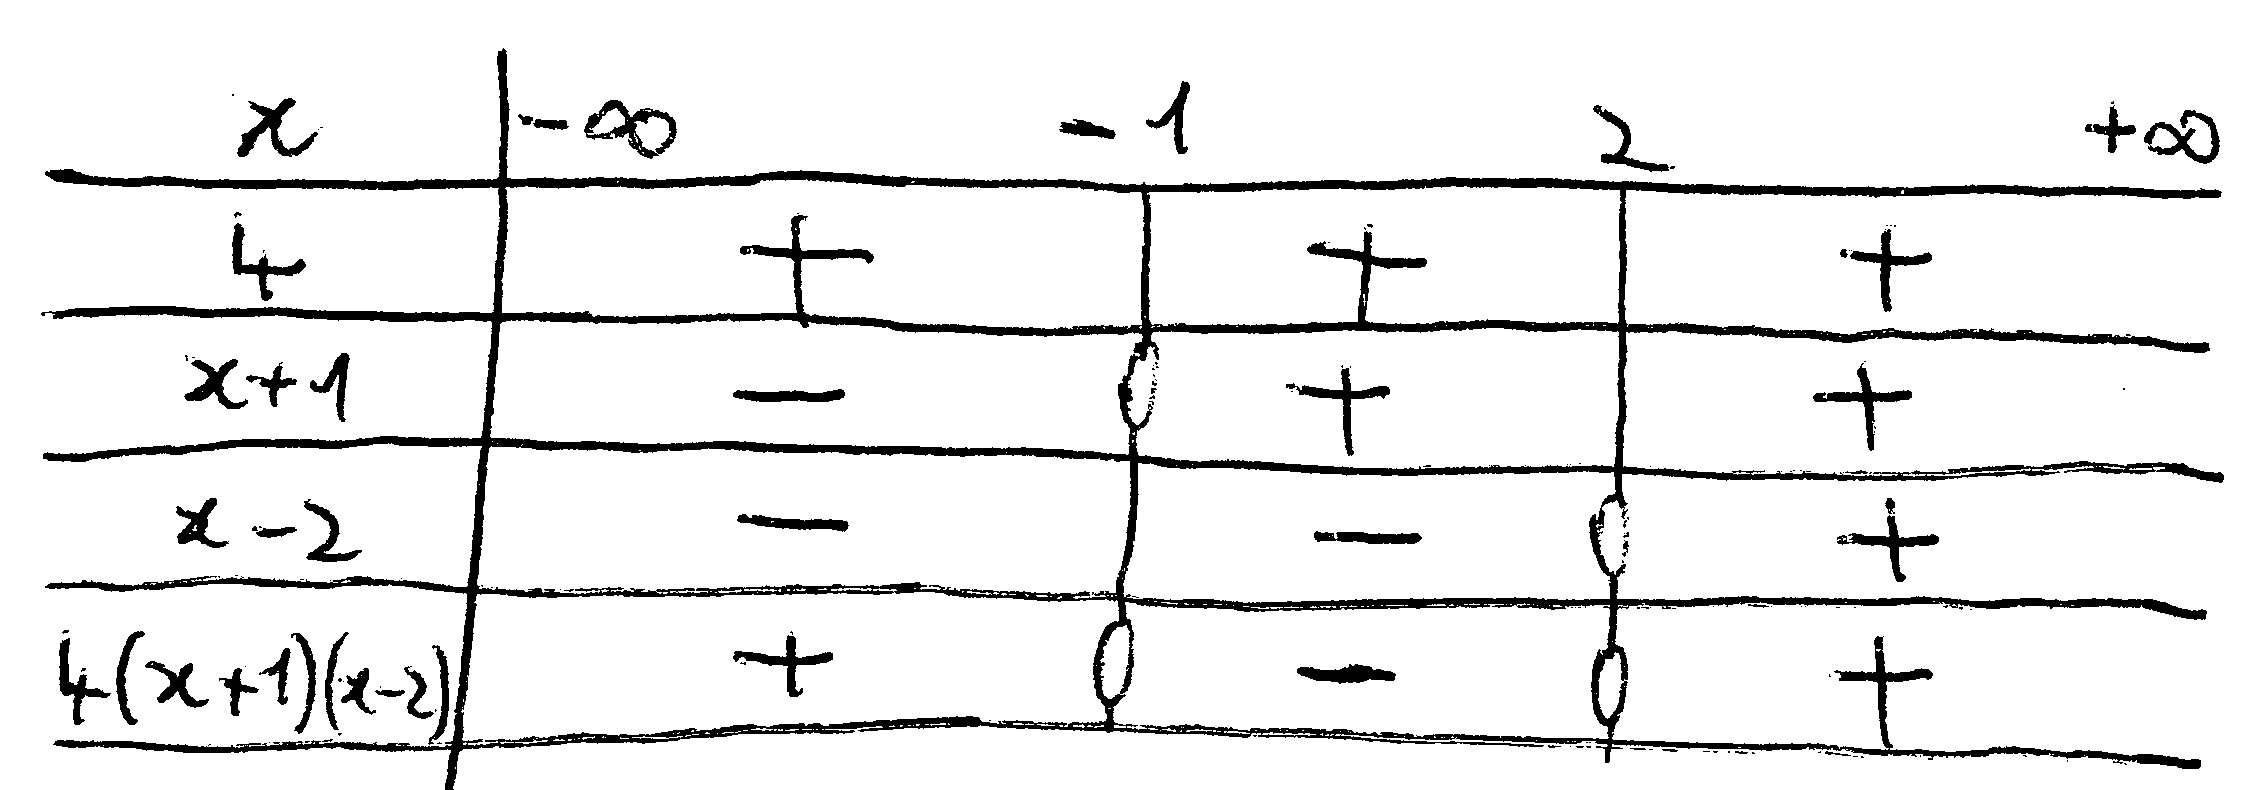
\includegraphics[width=0.4\textwidth]{pics/15.png}



D'où: $S = [-1;2]$.


\section*{Systèmes de 2 équations à 2 inconnues}

\exo{Résoudre les systèmes suivants:}

Lors de la résolution de ces systèmes, la résolution proposée est une parmi d'autres possibles. 

\question{$
\begin{cases}
3x+2y &= 42\\ 
2x+y &= 6
\end{cases}$}

On multiplie la 2\textsuperscript{ème} ligne par -2 afin d'annuler l'inconnue $y$ par addition.

$
\begin{cases}
3x+2y &= 42\\ 
-4x-2y &= -12
\end{cases}$

On obtient $-x = 30 \Leftrightarrow x = -30$.

On remplace ensuite dans une des 2 équations du système de départ:

$$3 \times (-30) +2y = 42 \Leftrightarrow 2y = 132 \Leftrightarrow y = 66$$

On obtient donc $x=-30$, $y=66$

\question{$
\begin{cases}
a+b &= 3\\ 
4a-b &= 2
\end{cases}$}

On peut directement additionner les deux lignes, ce qui va annuler la variable $b$:

On obtient $5a = 5 \Leftrightarrow a = 1$.

On remplace ensuite dans une des 2 équations du système de départ:

$$1+b = 3 \Leftrightarrow b = 2$$

On obtient donc $a=1$, $b=2$

\question{$
\begin{cases}
4v+6w &= -10\\ 
2v+w &= -1
\end{cases}$}

On multiplie la 2\textsuperscript{ème} ligne par -2 afin d'annuler l'inconnue $v$ par addition.

$
\begin{cases}
4v+6w &= -10\\ 
-4v-2w &= -2
\end{cases}$

On obtient $4w = -12 \Leftrightarrow w = -3$.

On remplace ensuite dans une des 2 équations du système de départ:

$$4v + 6 \times (-3) = -10 \Leftrightarrow 4v = 8 \Leftrightarrow v = 2$$

On obtient donc $v=2$, $w=-3$

\question{$
\begin{cases}
3\alpha+8\beta &= 2\\ 
2\alpha+7\beta &= 3
\end{cases}$}

On multiplie la 1\textsuperscript{re} ligne par -2 afin d'annuler l'inconnue $\alpha$ par addition.

$
\begin{cases}
-6\alpha-16\beta &= -4\\ 
6\alpha+21\beta &= 9
\end{cases}$

On obtient $5\beta = 5 \Leftrightarrow \beta = 1$.

On remplace ensuite dans une des 2 équations du système de départ:

$$3 \alpha + 8 \times 1 = 2 \Leftrightarrow 3 \alpha = -6 \Leftrightarrow \alpha = -2$$

On obtient donc $\alpha=-2$, $\beta=1$

\question{$
\begin{cases}
x+2y &= 2\\ 
\frac{x}{2}+y &= 3
\end{cases}$}

On multiplie la 2\textsuperscript{ème} ligne par -2 afin d'annuler l'inconnue $x$ par addition.

$
\begin{cases}
x+2y &= 2\\ 
x+2y &= 6
\end{cases}$

En additionnant les 2 lignes, on obtient $0 = 8$. Ce système n'a donc pas de solution. 

\question{$
\begin{cases}
3x+y &= 2\\ 
-6x-2y &= -4
\end{cases}$}

On multiplie la 1\textsuperscript{re} ligne par -2 afin d'annuler l'inconnue $x$ par addition.

$
\begin{cases}
-6x-2y &= -4\\ 
-6x-2y &= -4
\end{cases}$

On voit ici que les 2 équations sont équivalentes et on obtient par addition $0=0$. 

Il y a donc une infinité de solutions.


\exo{Véhicules}

%Un parking contient 35 véhicules. Des tricycles et des voitures (4 roues donc). Le nombre total de roues dans le parking est de 132. 

%Combien y a-t-il de véhicules de chaque type?

On appelle $t$ le nombre de tricycles et $v$ le nombre de voitures.

Il y a 2 inconnues, il nous faut donc trouver 2 équations. 

On sait qu'il y a au total 35 véhicules tout compris. On a donc $t+v = 35$.

Ensuite concernant le nombre de roues, chaque tricycle apporte 3 roues et chaque voiture en apporte 4. On obtient donc l'équation suivante: $3t + 4v = 132$.

On obtient donc le système suivant:

$
\begin{cases}
t+v &= 35\\ 
3t + 4v &= 132
\end{cases}$

On le résout comme lors de la série précédente: 

On multiplie la 1\textsuperscript{re} ligne par -3 et la 2\textsuperscript{ème} ligne par 3 afin d'annuler l'inconnue $t$ par addition.

$
\begin{cases}
-3t-3v &= -105\\ 
3t + 4v &= 132
\end{cases}$

On obtient $v = 27$.

On remplace ensuite dans une des 2 équations du système de départ:

$t + 28 = 35 \Leftrightarrow t = 7$.

Le parking contient donc 27 voitures et 8 tricycles.

\exo{Droites}

\question{Quelle est l'équation de la droite $(D_1)$ passant par les points $M_1(-2;-20)$ et $M_2(4;22)$ ?}

On rappelle que la forme générale de l'équation d'une droite s'écrit $y = ax+b$. Donner l'équation revient donc à trouver $a$ et $b$ qui seront les inconnues de notre système. Chaque point donné par lequel passe la droite correspond à un couple $(x;y)$ et va donner une équation. Le point $M_1 (-2;-20)$ nous donne l'équation $-2a + b = -20$ et le point $M_2 (4;22)$ nous donne l'équation $4a + b = 22$.

On peut donc écrire le système suivant:

$
\begin{cases}
-2a + b &= -20\\ 
4a + b &= 22
\end{cases}$

Que l'on résout comme on sait faire, par exemple en multipliant la première ligne par 2 afin d'éliminer l'inconnue $a$: 

$
\begin{cases}
-4a + 2b &= -40\\ 
4a + b &= 22
\end{cases}$

On obtient $3b = -18$ soit $b = -6$. 

On remplace $b$ par sa valeur dans la 2ème équation (par exemple): $4a - 6 = 22 \Leftrightarrow 4a = 28$.

Finalement, $a = 7$. 

L'équation de $(D_1)$ est donc $y = 7x - 6$. 

On peut écrire de façon plus synthétique: $(D_1):y = 7x - 6$.

\question{Et l'équation de $(D_2)$, qui elle passe par les points $N_1(2;2)$ et $N_2(-4;-1)$ ?}

De la même façon concernant la droite $(D_2)$, on obtient le système suivant:

$
\begin{cases}
2a + b &= 2\\ 
-4a + b &= -1
\end{cases}$

En multipliant la première ligne par 2:

$
\begin{cases}
4a + 2b &= 4\\ 
-4a + b &= -1
\end{cases}$

En additionnant les 2 lignes, on obtient $3b = 3 \Leftrightarrow b = 1$.

On remplace $b$ par sa valeur dans la première équation (on choisit celle dans laquelle les calculs seront les plus simples): $2a + 1 = 2 \Leftrightarrow 2a = 1 \Leftrightarrow a = \dfrac{1}{2}$.

On a donc $a = \dfrac{1}{2}$ et $b = 1$.

On obtient donc l'équation de $(D_2)$: $(D_2):y = \dfrac{1}{2}x + 1$.

\question{Quelles sont les coordonnées du point $I = (D_1) \cap (D_2)$ (qui est l'intersection des 2 droites)?}

On a $(D_1):y = 7x - 6$ et $(D_2):y = \dfrac{1}{2}x + 1$. Il s'agit de trouver le point d'intersection $I$ de ces deux droites. Les coordonnées $(x_I;y_I)$ de $I$ vérifient à la fois l'équation de $(D_1)$ et de $(D_2)$. Elles sont donc les solutions du système suivant:

$
\begin{cases}
y_I &= 7x_I - 6\\ 
y_I &= \dfrac{1}{2}x_I + 1
\end{cases}$

On peut multiplier la seconde ligne par -1 afin d'éliminer $y_I$.

$
\begin{cases}
y_I &= 7x_I - 6\\ 
-y_I &= -\dfrac{1}{2}x_I - 1
\end{cases}$

Pour obtenir $0 = \dfrac{13}{2}x_I - 7 \Leftrightarrow \dfrac{13}{2}x_I = 7 \Leftrightarrow x_I = 7 \times \dfrac{2}{13} = \dfrac{14}{13}$.

On remplace $x_I$ par sa valeur dans la première équation. 

$y_I = 7 \times \dfrac{14}{13} - 6 = \dfrac{98}{13} - \dfrac{78}{13}$ 

On obtient: $$y_I = \dfrac{20}{13}$$

Le point $I$ a donc pour coordonnées $\left( \dfrac{14}{13} ; \dfrac{20}{13} \right)$.

%\end{multicols}
\trait

\begin{center}
Fin.
\end{center}

\end{document}
